%----------------------------------------------------------------------------------------
%	CHAPTER Gesture Recognition Introduction
%----------------------------------------------------------------------------------------
\chapterimage{gesture.jpg} % Chapter heading image
\chapter{Gesture Recognition}
\section{Introduction}\index{Introduction}
About the history and the origin of GR, the purpose for gesture recognition. The 
introduction will also contain the reason why we will introduce the following algorithms.\bigskip


\section{Static Gestures}\index{Static Gestures}
This chapter includes the work done to detect static gestures. It begins by describing the general idea of segmentation and recognition and then proceeds to the following sections.\bigskip


\subsection{Prior Elaboration}\index{Prior Elaboration}
Segmentation is a very critical process. It depends majorly, in our case, on the detection of the hand, only the hand. That is why the lightest amount of noise could affect and diverge the result greatly. This is the reason behind noise elimination. It is an essential step prior to any segmentation process. We need to elaborate the image cleanly for the detector to easily find the item of interest among any other item in the image. Smoothing is considered the most effective solution in case of noise elimination. Many approaches have been devised to perform smoothing capably on the images just to keep the meaningful item for us unharmed in case there is any interference of any noise. The mask, filter, we use for noise elimination is Gaussian Smoothing.
need.\bigskip
\subsubsection{Gaussian Smoothing}\index{Prior Elaboraion}
The Gaussian smoothing operator is a 2-D convolution operator that is used to `blur' images and remove detail and noise. In this sense, it is similar to the mean filter, but it uses a different kernel that represents the shape of a Gaussian (`bell-shaped') hump. This kernel has some special properties which are detailed below.
\begin{figure*}[]
\begin{dBox}
\centering
  \mbox{
      \subfigure[Gaussian Distribution]{
            \label{fig:gaussian_1}
            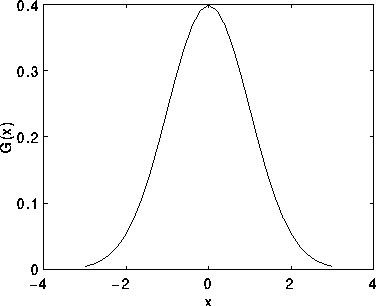
\includegraphics[width=.31\textwidth]{./Pictures/gesture/gaussian_distr.jpg}
        }
        \subfigure[Gaussian Distribution in 2D]{
           \label{fig:gaussian_2}
           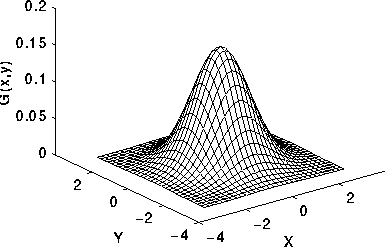
\includegraphics[width=.31\textwidth]{./Pictures/gesture/gaussian_distr_2d.png}
        }
   }
   \caption{Gaussian Distributions \label{fig:gaussian_dist} }   
\end{dBox}   
\end{figure*}
\bigskip
The Gaussian distribution in 1-D has the form:
\begin{dBox}
\begin{equation}
	G(x) = \frac{1}{\sqrt{2\pi\sigma}}e^{-\frac{x^2}{2\sigma^2}}
\end{equation}
\end{dBox}
where $\sigma$  is the standard deviation of the distribution. We have also assumed that the distribution has a mean of zero (i.e. it is centered on the line x=0). The distribution is illustrated in Figure \ref{fig:gaussian_dist}.
\bigskip
In 2-D, an isotropic (i.e. circularly symmetric) Gaussian has the form:
\begin{dBox}
\begin{equation}
	G(x,y) = \frac{1}{\sqrt{2\pi\sigma^2}}e^{-\frac{x^2+y^2}{2\sigma^2}}
\end{equation}
\end{dBox}
This distribution is shown in Figure \ref{fig:gaussian_dist}
\bigskip
The idea of Gaussian smoothing is to use this 2-D distribution as a `point-spread' function, and this is achieved by convolution. Since the image is stored as a collection of discrete pixels, we need to produce a discrete approximation to the Gaussian function before we can perform the convolution. In theory, the Gaussian distribution is non-zero everywhere, which would require an infinitely large convolution kernel, but in practice, it is effectively zero more than about three standard deviations from the mean, and so we can truncate the kernel at this point. Figure 3 shows a suitable integer-valued convolution kernel that approximates a Gaussian with a $\sigma$ of 1.0. It is not obvious how to pick the values of the mask to approximate a Gaussian.
%NOT FINISHED....................................
One could use the value of the Gaussian at the center of a pixel in the mask, but this 
is not accurate because the value of the Gaussian varies non-linearly across the pixel. We 
integrated the value of the Gaussian over the whole pixel (by summing the Gaussian at 0.001 
increments). The integrals are not integers: we rescaled the array so that the corners had the value 
1. Finally, the 273 is the sum of all the values in the mask. \bigskip

Once a suitable kernel has been calculated, then the Gaussian 
smoothing can be performed using standard convolution methods. 
The convolution can, in fact, be performed quickly since the 
equation for the 2-D isotropic Gaussian shown above is separable 
into x and y components. Thus, the 2-D convolution can be 
performed by first convolving with a 1-D Gaussian in 
the X direction, and then convolving with another 1-D Gaussian in 
the Y direction. (The Gaussian is in fact the only completely 
circularly symmetric operator that can be decomposed in such a 
way). 
%%%%%%%%%%%%%%%%%%%%%%%%%%%%%%%%%%%%%%%%%%%%%%%%%%%%%%
Figure \ref{fig:fig4} shows the 1-D x component kernel that would be used to produce the full kernel 
shown in Figure \ref{fig:fig3} (after scaling by 273, rounding and truncating one row of pixels around the 
boundary because they mostly have the value 0. This reduces the 7x7 matrix to the 5x5 shown 
above.). The Y component is exactly the same but is oriented vertically.

\begin{figure*}[h]
\begin{dBox}
\centering
  \mbox{
	    \subfigure[The full kernel]{
	          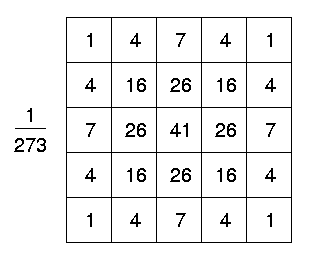
\includegraphics[width=.30\textwidth]{./Pictures/gesture/gaussian_kernal.png}
        }
   }
   \label{fig:fig3}   
\end{dBox}   
\end{figure*}

\begin{figure*}[h]
\begin{dBox}
\centering
  \mbox{
	    \subfigure[1-D x component kernel]{
	          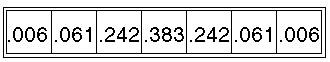
\includegraphics[width=.60\textwidth]{./Pictures/gesture/row_table.jpg}
        }
   }
   \caption{ \label{fig:fig4} }   
\end{dBox}   
\end{figure*}


\bigskip
A further way to compute a Gaussian smoothing with a large 
standard deviation is to convolve an image several times with a 
smaller Gaussian. While this is computationally complex, it can have applicability if the processing 
is carried out using a hardware pipeline. 
\bigskip
The Gaussian filter not only has utility in engineering applications. It is also attracting attention 
from computational biologists because it has been attributed with some amount of biological 
plausibility, e.g. some cells in the visual pathways of the brain often have an approximately 
Gaussian response.

\bigskip
The effect of Gaussian smoothing is to blur an image, in a similar fashion to the mean filter. The 
degree of smoothing is determined by the standard deviation of the Gaussian. (Larger standard 
deviation Gaussians, of course, require larger convolution kernels in order to be accurately 
represented.) 

\bigskip
The Gaussian outputs a `weighted average' of each pixel's neighborhood, with the average 
weighted more towards the value of the central pixels. This is in contrast to the mean filter's 
uniformly weighted average. Because of this, a Gaussian provides gentler smoothing and 
preserves edges better than a similarly sized mean filter. 
\bigskip

One of the principle justifications for using 
the Gaussian as a smoothing filter is due 
to its frequency response. Most 
convolution-based smoothing filters act as 
lowpass frequency filters. This means that 
their effect is to remove high spatial 
frequency components from an image. The 
frequency response of a convolution 
filter, i.e. its effect on different spatial 
frequencies, can be seen by taking the 
Fourier transform of the filter. Figure \ref{fig:fig5}
shows the frequency responses of a 1-D mean filter with width 5 and also of a Gaussian filter 
with $\sigma$ = 3. We used figure \ref{fig:fig6} to illustrate the Gaussian’s smoothing effect.

\begin{figure*}[h]
\begin{dBox}
\centering
  \mbox{
	    \subfigure[Frequency responses]{
	          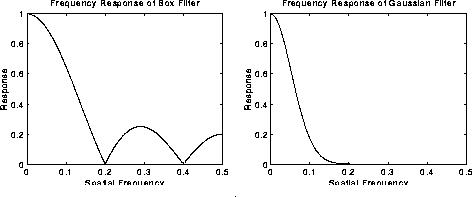
\includegraphics[width=.80\textwidth]{./Pictures/gesture/freq_responses.jpg}
        }
   }
   \caption{Frequency responses \label{fig:fig5} }   
\end{dBox}   
\end{figure*}

\begin{figure*}[h]
\begin{dBox}
\centering
  \mbox{
      \subfigure[]{
            \label{fig:smooth1}
            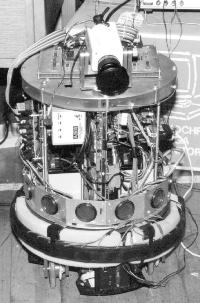
\includegraphics[width=.31\textwidth]{./Pictures/gesture/smooth1.jpg}
        }
        \subfigure[]{
           \label{fig:smooth2}
           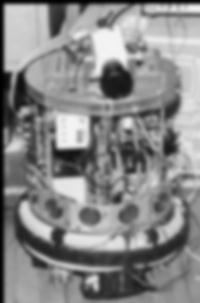
\includegraphics[width=.31\textwidth]{./Pictures/gesture/smooth2.jpg}
        }
        \subfigure[]{
            \label{fig:sift_3}
            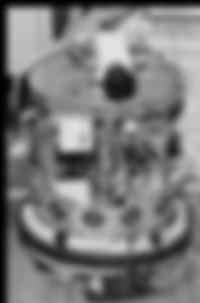
\includegraphics[width=.31\textwidth]{./Pictures/gesture/smooth3.jpg}
       }
   }
   \caption{Gaussian’s smoothing effect \label{fig:fig6} }   
\end{dBox}   
\end{figure*}


We used an appropriate value for $\sigma$ and a kernel size 5*5 in our work. Of course, the higher 
kernel size we provide, the better smoothing we get, but the problem resides in the processing 
overhead. Since we have more processing coming head in several parts coming ahead we cannot 
just strain it and delay it here. Therefore, a secured limit of smoothing is sufficient to avoid the 
results that could harm the further work coming ahead. 
\bigskip


\subsubsection{Color Segmentation }\index{Color Segmentation }
Color image segmentation is useful in many applications. From the segmentation results, it is 
possible to identify regions of interest and objects in the scene, which is very beneficial to the 
subsequent image analysis or annotation. The problem of segmentation is difficult because of 
image texture. If an image contains only homogeneous color regions, clustering methods in color 
space are sufficient to handle the problem. In reality, natural scenes are rich in color and texture. 
It is difficult to identify image regions containing color-texture patterns.\bigskip

Color images are usually represented in terms of their Red, Green and Blue components (RGB 
format) for purposes of storage and display. All of the color spaces can be derived from the RGB 
information supplied by devices such as cameras and scanners. The RGB color space is the most 
prevalent choice for computer graphics because color displays use red, green, and blue to create 
the desired color. Therefore, the choice of the RGB color space simplifies the architecture and 
design of the system. Furthermore, a system that is designed using the RGB color space can 
take advantage of a large number of existing software routines, since this color space has been 
around for a number of years.  \bigskip

However, RGB is not very efficient when dealing with “real-world” images. All three RGB 
components need to be of equal bandwidth to generate any color within the RGB color cube. 
The result of this is a frame buffer that has the same pixel depth and display resolution for each RGB component. In addition, processing an image in the RGB color space is usually not the 
most efficient method. For example, to modify the intensity or color of a given pixel, the three 
RGB values must be read from the frame buffer, the intensity or color calculated, the desired 
modifications performed, and the new RGB values calculated and written back to the frame 
buffer. If the system had access to an image stored directly in the intensity and color format, 
some processing steps would be faster. That is why we need desperately to move from RGB to 
another domain, where segmentation is more reliable. We have found it most beneficial to 
convert to YCBCr color space. \bigskip

The YCbCr color space is widely used for digital video. In this format, luminance information is 
stored as a single component (Y), and chrominance information is stored as two color-difference 
components (Cb and Cr). Cb represents the difference between the blue component and a 
reference value. Cr represents the difference between the red component and a reference value. \bigskip


YCbCr data can be double precision, but the color space is particularly well suited 
to uint8 data. For uint8 images, the data range for Y is [16, 235], and the range for Cb and Cr is 
[16, 240]. YCbCr leaves room at the top and bottom of the full uint8 range so that additional 
(nonimage) information can be included in a video stream. From YCbCr we apply a threshold 
on this color space to convert the image to the grayscale image.\bigskip

The resulting conversion, based on a threshold, may result in a noise that we don’t desire them 
to exist. This noise is totally hazard to the further processing of the image. Which means that 
we need another smoothing step. This time the smoothing requires us to preserve certain details 
in the image, which are the edges of our items of interest. Consequently, we need a conservative 
smoothing that could secure us to preserve edges, which introduces us to the median filter.\bigskip

\subsubsection{Conservative Smoothing (Median Filter)} \index{Conservative Smoothing (Median Filter)}
Conservative smoothing is a noise reduction technique that derives its name from the fact that it 
employs a simple, fast filtering algorithm that sacrifices noise suppression power in order to 
preserve the high spatial frequency detail (e.g. sharp edges) in an image. It is explicitly designed 
to remove noise spikes --- i.e. isolated pixels of exceptionally low or high pixel intensity (e.g. salt 
and pepper noise) and is, therefore, less effective at removing additive noise (e.g. Gaussian noise) 
from an image.  \bigskip

Like most noise filters, conservative smoothing operates on the assumption that noise has a 
high spatial frequency and, therefore, can be attenuated by a local operation which makes each 
pixel's intensity roughly consistent with those of its nearest neighbors. However, whereas mean 
filtering accomplishes this by averaging local intensities and median filtering by a non-linear 
rank selection technique, conservative smoothing simply ensures that each pixel's intensity is 
bounded within the range of intensities defined by its neighbors.  \bigskip

The median filter is normally used to 
reduce noise in an image, somewhat 
like the mean filter. However, it often 
does a better job than the mean filter 
of preserving useful detail in the 
image. Like the mean filter, the 
median filter considers each pixel in 
the image in turn and looks at its 
nearby neighbors to decide whether or 
not it is representative of its 
surroundings. Instead of simply replacing the pixel value with the mean of neighboring pixel 
values, it replaces it with the median of those values. The median is calculated by first sorting 
all the pixel values from the surrounding neighborhood into numerical order and then replacing 
the pixel being considered with the middle pixel value. (If the neighborhood under consideration 
contains an even number of pixels, the average of the two middle pixel values is used.) Figure \ref{fig:fig7}
illustrates an example calculation.

\begin{figure*}[h]
\begin{dBox}
\centering
\mbox{
	    \subfigure[]{
	          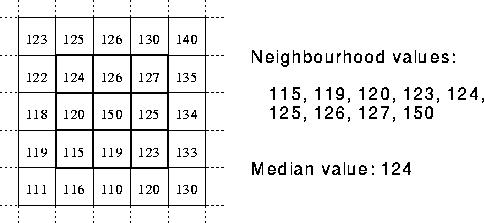
\includegraphics[width=.80\textwidth]{./Pictures/gesture/median.jpg}
        }
   }
   \caption{
   \label{fig:fig7} }   
\end{dBox}   
\end{figure*}
\bigskip

By calculating the median value of a neighborhood rather than the mean filter, the median filter 
has two main advantages over the mean filter: 
\begin{itemize}
\item The median is a more robust average than the mean and so a single very 
unrepresentative pixel in a neighborhood will not affect the median value significantly. 
\item Since the median value must actually be the value of one of the pixels in the 
neighborhood, the median filter does not create new unrealistic pixel values when the 
filter straddles an edge. For this reason, the median filter is much better at preserving 
sharp edges than the mean filter.
\end{itemize}

Figure \ref{fig:fig8} illustrates the effect of the median filter with many kernel sizes. At our 
work, we used the median filter with kernel size 5*5. It was most convenient for our work and 
this size preserved the edges the way we would like it to be. 
\begin{figure*}[h]
\begin{dBox}
\centering
  \mbox{
      \subfigure[]{
            \label{fig:sift_1}
            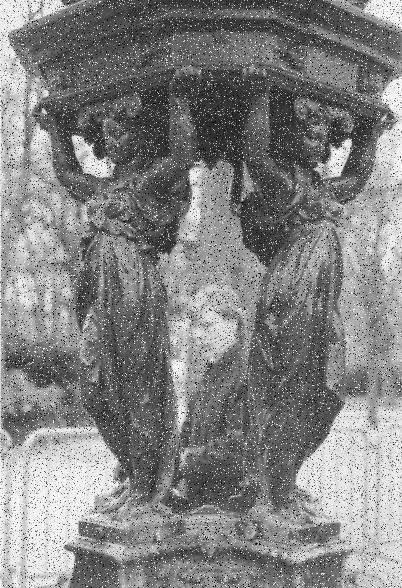
\includegraphics[width=.31\textwidth]{./Pictures/gesture/smooth_median_1.jpg}
        }
        \subfigure[]{
           \label{fig:sift_2}
           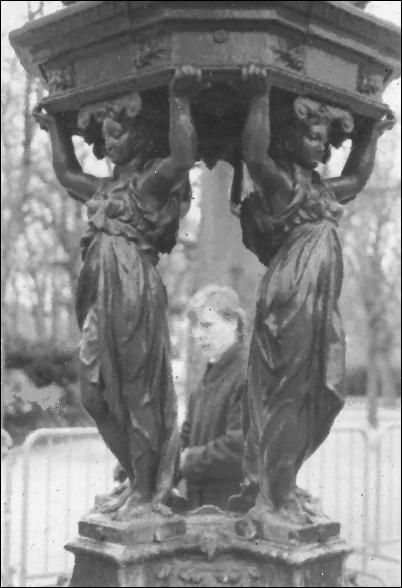
\includegraphics[width=.31\textwidth]{./Pictures/gesture/smooth_median_2.jpg}
        }
        \subfigure[]{
            \label{fig:sift_3}
            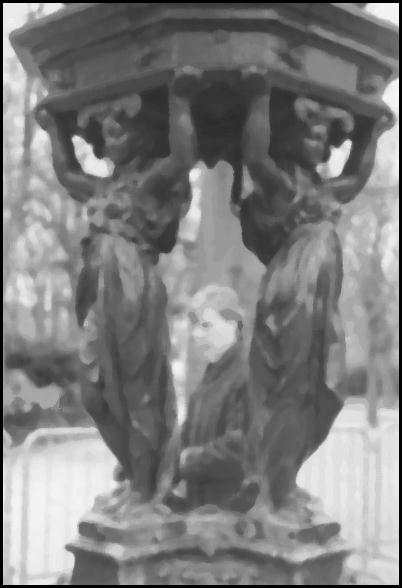
\includegraphics[width=.31\textwidth]{./Pictures/gesture/smooth_median_3.jpg}
       }
   }
   \caption{Median Filter \label{fig:fig8} }   
\end{dBox}   
\end{figure*}

\subsubsection{Binary Image and Connected Components}\index{Binary Image and Connected Components}
NOT YET !!!!!!!!!!!!!!!!!!!!!!!!!!!!!!!!!!!!!!!!!!!!!!!!!!!!!!!!!!!!!!!!!!!!!!!!!!!!


\subsection{Algorithm One: Predefined Features Extraction}\index{Algorithm One: Predefined Features Extraction}
Feature extraction is a crucial step in computer vision applications for hand gesture recognition. The pre-processing stage prepares the input image and extracts features used later with the classification algorithms. This set of features shall be unique per ever gesture. The set of features the algorithm generates for training the dataset are as follow:
\bigskip
\begin{itemize}
\item Mean and Variance of the gray pixel values.
\item The hand area and perimeter.
\item Hand orientation.
\item Orientation histogram.
\item Radial signature.
\end{itemize}
\bigskip
\begin{figure*}[]
\begin{dBox}
\centering
  \mbox{
      \subfigure[Mean and variance]{
            \label{fig:mean_var}
            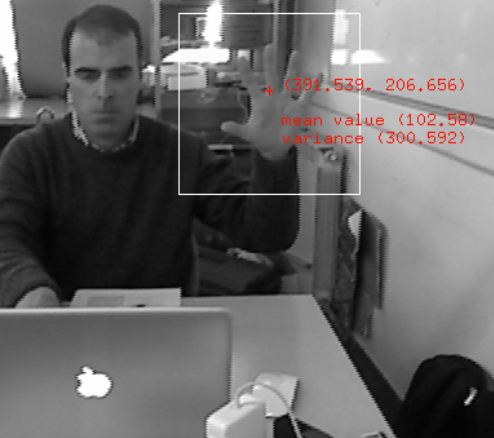
\includegraphics[width=.31\textwidth]{./Pictures/gesture/mean_var.jpg}
        }
        \subfigure[Area and perimter]{
           \label{fig:area}
           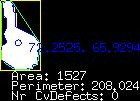
\includegraphics[width=.31\textwidth]{./Pictures/gesture/area.jpg}
        }
   }
   \caption{First Two Features \label{fig:mean_area} }   
\end{dBox}   
\end{figure*}
\bigskip
The first two features: mean, variance and the blob area and perimeter are detected from the previous steps prior to the algorithm. The smoothing followed by obtaining the gray image helps us finding the mean and the variance of the gray pixel values that represent the blob according to figure \ref{fig:mean_area}. The blob area and perimeter are detected from the last elaboration step which is finding the binary image for the blob. Figure \ref{fig:mean_area} illustrates how this works. The area of the white region is calculated approximated and then the perimeter is determined on the position of the hand on the image. This now leaves us with the rest of the five other features remaining to find in the set.
\bigskip
\subsubsection{Hand Orientation}\index{Algorithm One: Predefined Features Extraction}
The segmented hand is used to calculate its orientation with the help of image moments. Moment approximations provide one of the more obvious means of describing 2-D shapes. The moments involve sums over all pixels, and so are robust against small pixel changes. If I x, y is the image intensity at position x and y then the image moments, up to the second order, are:
\bigskip
\begin{dBox}
\begin{equation}
	M_{00}= \sum_{x}\sum_{y}I(x,y)
\end{equation}
\begin{equation}
	M_{01}= \sum_{x}\sum_{y}y.I(x,y)
\end{equation}
\begin{equation}
	M_{10}= \sum_{x}\sum_{y}x.I(x,y)
\end{equation}
\begin{equation}
	M_{11}= \sum_{x}\sum_{y}xy.I(x,y)
\end{equation}
\begin{equation}
	M_{20}= \sum_{x}\sum_{y}x^{2}I(x,y)
\end{equation}
\begin{equation}
	M_{02}= \sum_{x}\sum_{y}y^{2}I(x,y)
\end{equation}
\end{dBox}
\bigskip
The hand position can be calculated as follows:
\bigskip
\begin{dBox}
\begin{equation}
	x_{c} = \frac{M_{10}}{M_{00}}
\end{equation}
\begin{equation}
	y_{c} = \frac{M_{01}}{M_{00}}
\end{equation}
\end{dBox}
\bigskip
The hand orientation can then be calculated using the following intermediate variables a, b and c:
\bigskip
\begin{dBox}
\begin{equation}
	a = \frac{M_{20}}{M_{00}} - x_{c}^{2}
\end{equation}
\begin{equation}
	b = 2 (\frac{M_{10}}{M_{00}}-x_{c}y_{c})
\end{equation}
\begin{equation}
    c = \frac{M_{02}}{M_{00}}- y_{c}^{2}
\end{equation}
\end{dBox}
\bigskip
and the angle is:
\begin{dBox}
\begin{equation}
\theta = \frac{tan^{-1}(b,(a-c))}{2}
\end{equation}
\end{dBox}
\bigskip
\subsubsection{Orientation Histogram}\index{Algorithm One: Predefined Features Extraction}
Pixel intensities can be sensitive to lighting variations,
which lead to classification problems within the same gesture under different light conditions. The use of local
orientation measures avoids this kind of problem, and the
histogram gives us translation invariance. Orientation
histograms summarize how much of each shape is oriented in each possible direction, independent of the position of the hand inside the camera frame. This statistical technique is most appropriate for close-ups of the hand. In our work, the hand is extracted and separated from the background. This provides a uniform black background, which makes this statistical technique a good method for the identification of different static hand poses. This method is insensitive to small changes in the size of the hand, but it is sensitive to changes in hand orientation.\bigskip

We have calculated the local orientation using image gradients, represented by horizontal and vertical image pixel differences. If dx and dy are the outputs of the derivative operators, then the gradient direction is $arctan(dx,dy)$ and the contrast is  $\sqrt{d_{x}^{2}+d_{y}^{2}}$ A contrast threshold is set as some amount k times the mean image contrast, below which we assume the orientation measurement is inaccurate. A value of k=1.2 was used in the experiments. We then blur the histogram in the angular domain as in with a [1 4 6 4 1] filter, which gives a gradual fall-off in the distance between orientation histograms.\bigskip

Our histogram of orientation is composed of 36 bins, which means that this feature is described via 36 values.
\bigskip
\subsubsection{Radial Signature}\index{Algorithm One: Predefined Features Extraction}
A simple method to assess the gesture would be to measure the distance from the hand centroid to the edges of the hand along a number of radials equally spaced around a circle. This would provide information on the general “shape” of the gesture that could be easily rotated to account for hand yaw (since any radial could be used as datum).
\bigskip
Figure \ref{fig:radial_sig} (a) shows a gesture with example radials (simplified).
However, a problem (as shown in Figure \ref{fig:radial_sig} (a) ) is how to measure when the radial crosses a gap between fingers or between the palm and a finger. To remedy this it was decided to count the total number of skin pixels along a given radial. This is shown in Figure \ref{fig:radial_sig} (b). All of the radial measurements could then be scaled so that the longest radial was of constant length. By doing this, any alteration in the hand camera distance would not affect the radial length signature generated.

\begin{figure*}[h]
\begin{dBox}
\centering
  \mbox{
      \subfigure[Radial Idea]{
            \label{fig:radial}
            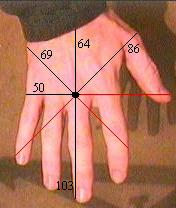
\includegraphics[width=.31\textwidth]{./Pictures/gesture/radial.jpg}
        }
        \subfigure[Corrected Radial]{
           \label{fig:radial_2}
           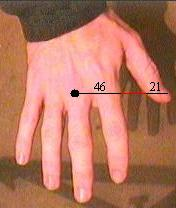
\includegraphics[width=.31\textwidth]{./Pictures/gesture/radial2.jpg}
        }
   }
   \caption{Radial Signature \label{fig:radial_sig} }   
\end{dBox}   
\end{figure*}

A simple method to assess the gesture would be to measure the distance from the hand centroid to the edges of the hand along a number of equally spaced radials. For the present feature extraction problem, 100 equally spaced radials were used. To count the number of pixels along a given radial we only take into account the ones that are part of the hand, eliminating those that fall inside gaps, like the ones that appear between fingers or between the palm and a finger.
\bigskip

During tests it was noticed that the quality of recognition depended on the number of radials used. It was also noticed that most of the significant data was concentrated around the fingers, thus it would be more efficient to group radials in these areas. Figure \ref{fig:radial_bins} shows the radials in their original grouping and after reorganization.
\bigskip
\begin{figure*}[h]
\begin{dBox}
\centering
  \mbox{
      \subfigure[Radial Signature with bin=100]{
            \label{fig:ori_bin}
            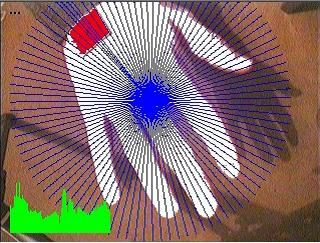
\includegraphics[width=.31\textwidth]{./Pictures/gesture/ori_bins.jpg}
        }
        \subfigure[Radial Signature with bin=100]{
           \label{fig:inc_bin}
           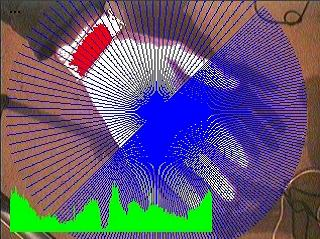
\includegraphics[width=.31\textwidth]{./Pictures/gesture/inc_bins.jpg}
        }
   }
   \caption{Radial Signature with different bin sizes \label{fig:radial_bins} }   
\end{dBox}   
\end{figure*}

All the radial measurements can be scaled so that the longest radial has a constant length. With this measure, we can have a radial length signature that is invariant to hand distance from the camera.
\subsection{Algorithm Two: Binary Representation}\index{Algorithm Two: Binary Representation}
The algorithm is based on describing the image, compare this description, and classify it with the help of the data set after walking through the previously mentioned steps for elaborating the image and extracting the hand in binary representation, an example for a binary image is shown in figure \ref{fig:open_binary}. Standardly, we now have an image that contains two meaningful details only the foreground pixels that should only represent the hand and the background pixels that only represent the background. Generally, to describe an image we need every pixel of image to declare itself, vote whether it is foreground or background, and then we can have the general visualization for the image by traversing ever pixel and checking what it looks like. Therefore, to traverse ever pixel this is a huge processing consumption given that we have many frames coming in it is needless to do a per pixel checking for each image in each frame. \bigskip
\begin{figure*}[h]
\begin{dBox}
\centering
  \mbox{
      \subfigure[Open Hand]{
            \label{fig:binary_op}
            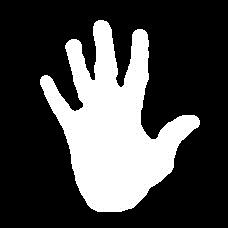
\includegraphics[width=.31\textwidth]{./Pictures/gesture/binary_open.jpg}
        }
       
        }
   \caption{Binary Image Example \label{fig:open_binary} }   
\end{dBox}   
\end{figure*}

Our algorithm alleviates such processing burden. The general idea of the algorithm includes this voting but in a less processing way. We need parts of the image to vote on their existence but not pixel by pixel. Given the binary image, it is quite visible that most of the pixels are going to declare themselves a background pixel or, at the best fitting, we find the same number of pixels on foreground and background. However, this is still a waste of processing. The algorithm we are about to detail its idea starts by introducing what can resolve this needless processing waste, the griding. \bigskip

\subsubsection{Griding The Binary Image}\index{Algorithm Two: Binary Representation}
Our Work begins by dividing the binary image we obtained from our elaboration steps into grids as shown in Figure \ref{fig:grid_idea}. The griding is an alternative approach for pixel-by-pixel traversing. In this approximation, we just process n grids, standardly, rather than over thousands and thousands of pixels. This solution is based on the nature of the input image as a binary image. It may not work if the image is not binary image. The binary representation helps us limit any grid value to either 0 or 1 according to the voting technique we use.\bigskip
\begin{figure*}[h]
\begin{dBox}
\centering
  \mbox{
      \subfigure[]{
            \label{fig:binary_op}
            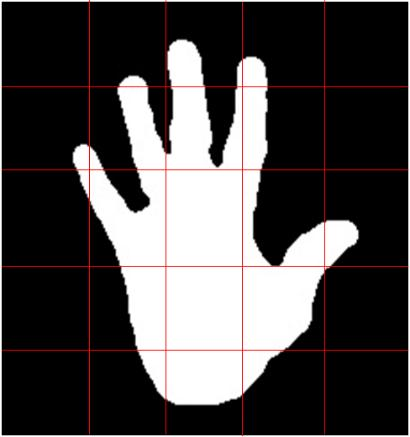
\includegraphics[width=.31\textwidth]{./Pictures/gesture/gridding_idea.jpg}
        }
       
        }
   \caption{Griding Idea Example \label{fig:grid_idea} }   
\end{dBox}   
\end{figure*}

\subsubsection{Grid Voting}\index{Algorithm Two: Binary Representation}
As the image is a binary image, some grids vote according to one of the following cases in Figure \ref{fig:vote_idea}
\begin{figure*}[h]
\begin{dBox}
\centering
  \mbox{
      \subfigure[]{
            \label{fig:vote_cases}
            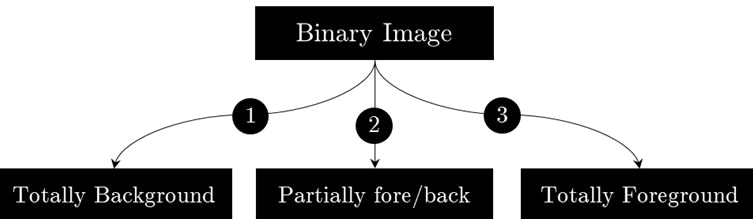
\includegraphics[width=.8\textwidth]{./Pictures/gesture/vote_cases.png}
        }
       
        }
   \caption{ Grids Vote Cases \label{fig:vote_idea} }   
\end{dBox}   
\end{figure*}
\paragraph{$1^{st}$ Case: Totally Background}\index{Grid Voting}
In this case, the whole grid is formed by background pixels only as shown in Figure \ref{fig:vote_cases_d} (a), all of them are black pixels. Consequently, the grid votes on its value to be 0. Note that to know this nature about a grid we traverse its pixels. This is not reverting us back to the pixel-by-pixel approach but, here, we just traverse until we encounter the existence of a one white pixel only. This white pixel is always interpreted as a foreground pixel and this moves us to the second case. Therefore, we are not traversing all the pixels this just happens in the grids that contain no foreground pixels but generally, the voting is determined after the traversing is done once we hit the end of the grid and no foreground pixels exist or once we come across a foreground pixel. Which guarantees the running time and the processing time to be kept lower than the former approach that counts the voting of ever pixel.
\begin{figure*}[h]
\begin{dBox}
\centering
  \mbox{
      \subfigure[Case 1]{
            \label{fig:black}
            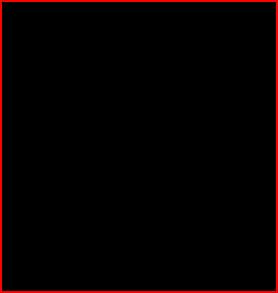
\includegraphics[width=.18\textwidth]{./Pictures/gesture/black_cell.jpg}
        }
        \subfigure[Case 2]{
           \label{fig:partial}
           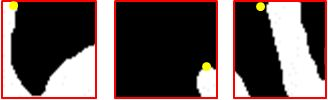
\includegraphics[width=.63\textwidth]{./Pictures/gesture/partially.jpg}
        }
        \subfigure[Case 3]{
           \label{fig:white}
           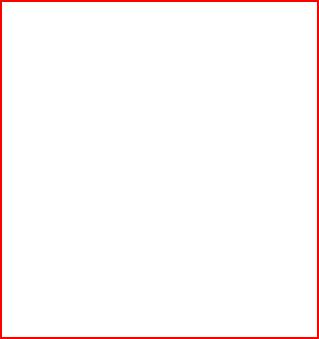
\includegraphics[width=.18\textwidth]{./Pictures/gesture/white_cell.jpg}
        }
   }
   \caption{Grid Shapes \label{fig:vote_cases_d} }   
\end{dBox}   
\end{figure*}

\paragraph{$2^{nd}$ Case: Partially Background}\index{Grid Voting}
Different from the first case, the image’s grid, in this one, encounters the presence of two kinds of pixels; background and foreground. Check examples in Figure \ref{fig:vote_cases_d}.
In this case, the voting is determined directly, without traversing, if the first pixel in the grid is a foreground pixel. However there could be a background pixels in the upcoming parts of the grid but we don’t need to traverse for the rest of pixels, as the voting immediately turns to “1” once we find this white pixel. Otherwise, if the first pixel is background pixel, hence, we begin in the same way as the first case until we hit the presence of a foreground pixel then the traversing is terminated and the vote of the whole grid turns to “1”. If no foreground pixels detected, then the voting remains “0” as in the first case. The grid that can be seen as an edge grid is the one that can be described via this case. The traversing stops at the yellow points which explains the variety of this case.
All these sub-cases are shown in Figure \ref{fig:vote_cases_d} (b).\bigskip
\paragraph{$3^{rd}$ Case: Totally Foreground}\index{Grid Voting}
There is no much difference between this case and the previous one. In both cases, we encounter the presence of foreground pixels but this case can be considered a special case from the previous case since we have no background pixels. Which means that the grid is totally foreground. This can be interpreted that the grid is not an edge grid, as it has nothing from the background. As show in Figure \ref{fig:vote_cases_d}(c).
The Whole case and the vote determination is explained by the flow chart in Figure \ref{fig:vfc}.
\begin{figure*}[h]
\begin{dBox}
\centering
  \mbox{
      \subfigure[]{
            \label{fig:binary_op}
            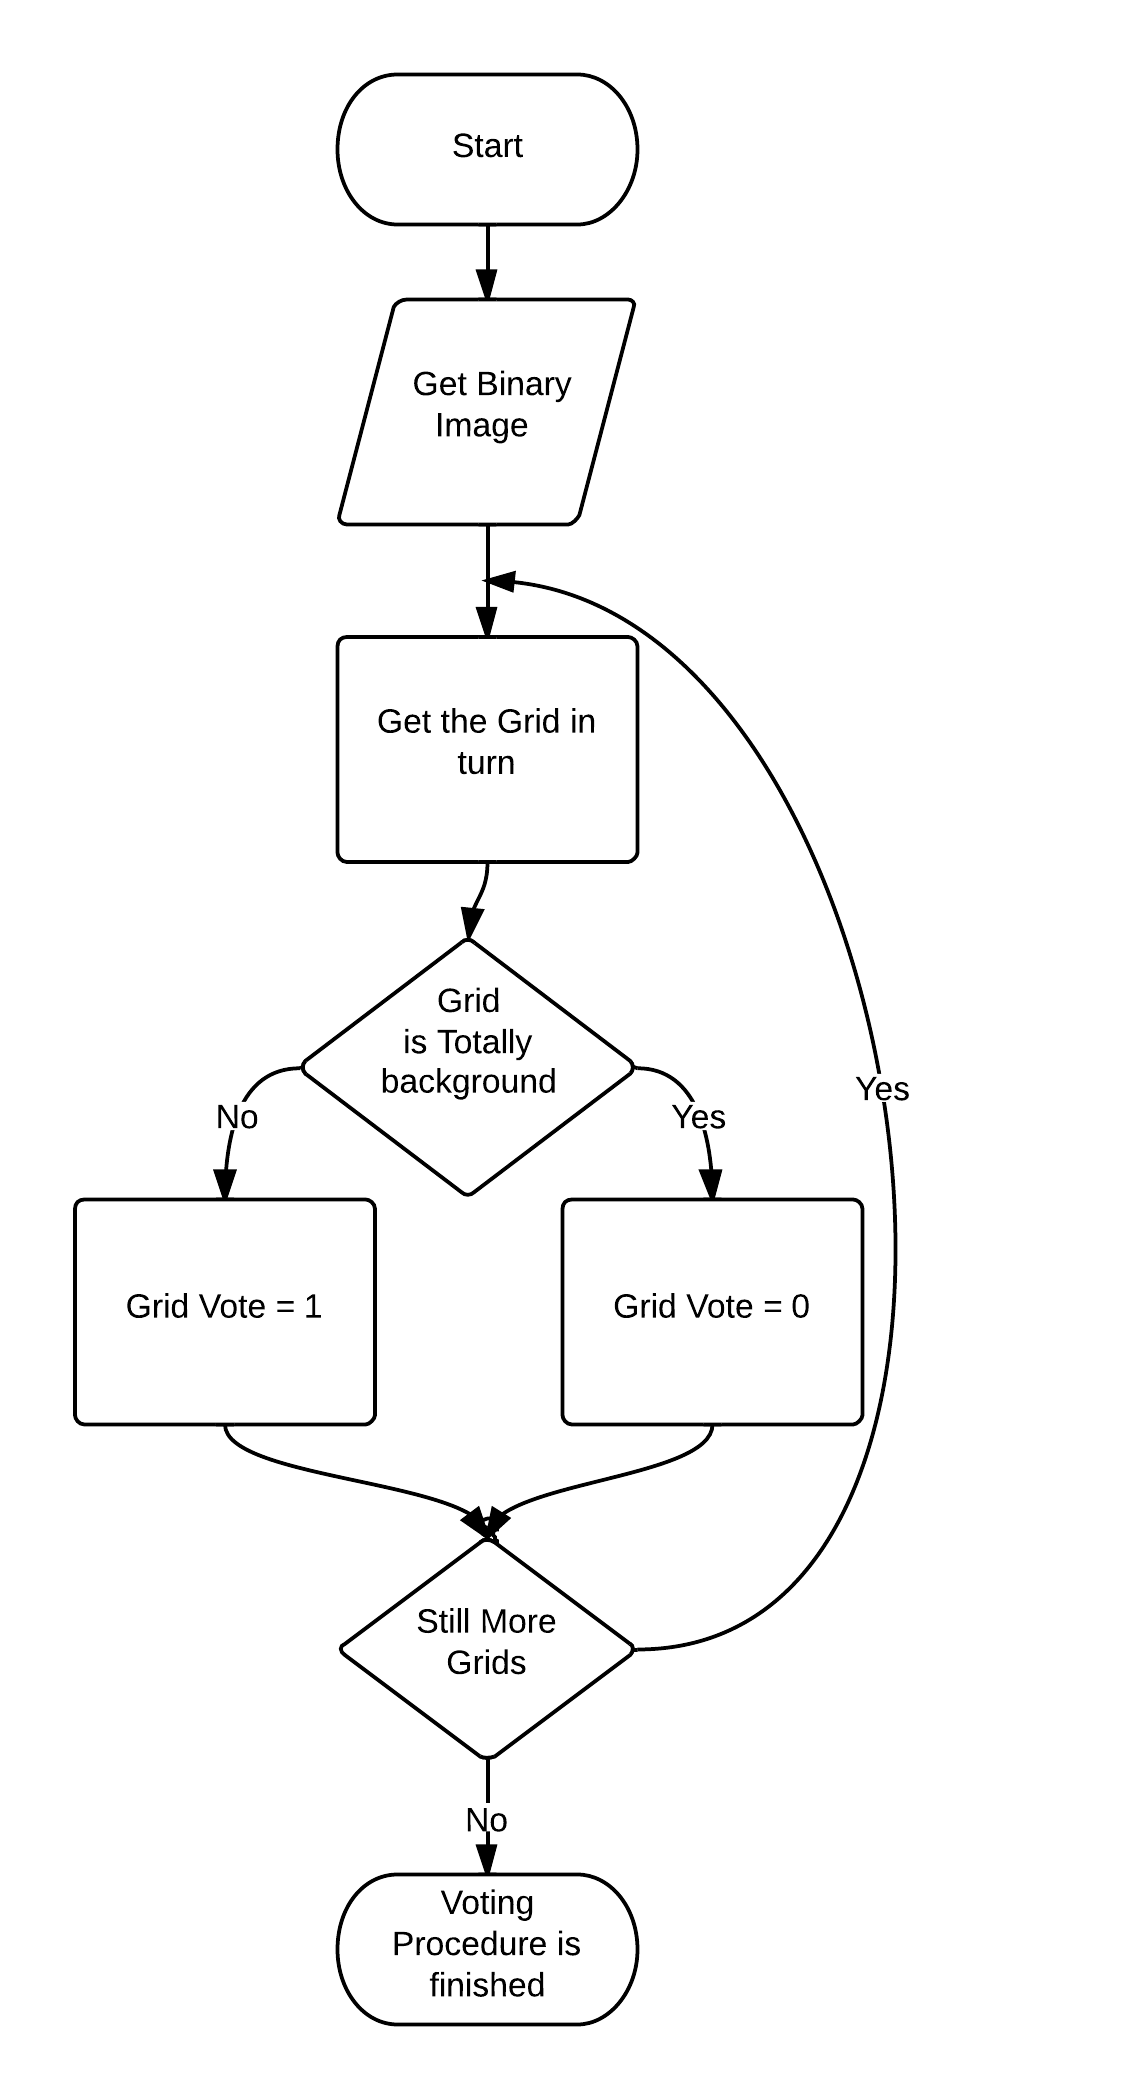
\includegraphics[width=.6\textwidth]{./Pictures/gesture/vfc.png}
        }
       
        }
   \caption{Voting Flow Chart \label{fig:vfc} }   
\end{dBox}   
\end{figure*}

The griding approximation is acting as if we let group of pixels decides rather than pixel by pixel. On the one hand, this counts best for the processing performance, much better, but on the other hand, that doesn’t sound promising for the accuracy. To illustrate this clearly let us consider and talk about the following example if we choose the griding to be only 2*2 grids. At this case, we may have the binary shape of the hand, in any form. While detection, it will always results in a just four grids and all of them are voted to be 1. Another case, if we used 5*5 grids. This results in a completely different voting result. Furthermore, if we used 10*10 grids, the resulting voting is presented in the Figure \ref{fig:bin_sizes} (a,b,c)
\begin{figure*}[h]
\begin{dBox}
\centering
  \mbox{
      \subfigure[n=2]{
            \label{fig:n2}
            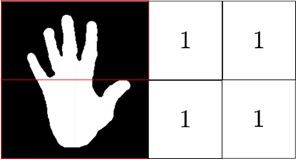
\includegraphics[width=.33\textwidth]{./Pictures/gesture/n2.jpg}
        }
        \subfigure[n=5]{
           \label{fig:n5}
           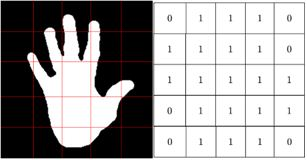
\includegraphics[width=.33\textwidth]{./Pictures/gesture/n5.jpg}
        }
        \subfigure[n=10]{
           \label{fig:n10}
           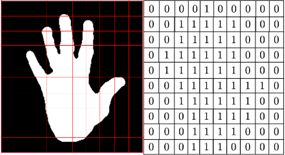
\includegraphics[width=.33\textwidth]{./Pictures/gesture/n10.jpg}
        }
   }
   \caption{Voting Results Using Different Grid Sizes \label{fig:bin_sizes} }   
\end{dBox}   
\end{figure*}

The pixel-by-pixel detection gives us an optimal description and yet the worst performance but we can approximate our approach to go nearer to this optimal description and yet preserves the performance. This can be achieved if we choose a larger number of grids that can actually be considered as if they are pixels not girds. The larger we keep the number of girds growing to be, the better accuracy we obtain, and the worse the performance gets. This keeps happening as long as we increase the number of girds until the grid is actually a pixel, then, the worst performance occur and the best accuracy is obtained.\bigskip

The reason why this happens can be see clearly in table (Not Yet). When we increase the grid size, we happen to include more details in each grid that can be described optimally and totally by pixel-by-pixel approach. As long as we make the grids come across edges in a way that griding attempts to preserve the shape of the binary image, our accuracy will rapidly grow. Therefore, to conclude, more girds better accuracy. Every time we enlarge the gird size we check the accuracy and performance until we hit this number of grids that gives acceptable results on each as recorded in table (Not Yet).\bigskip

The previous figures also assert what we were saying about the indispensability of noise elimination. Since, if we got one white noisy spot in the image it will significantly affect the resulting matrix and affect all that is following this step.
\subsubsection{Flatting The Votes}\index{Algorithm Two: Binary Representation}
After each gird’s voting is determined, now we get a matrix of 0s and 1s. This matrix will be formulated as 1-D array that Represent the feature array which will be passed to the classifier either for training/evaluating.

We get to detail how the classifiers we used to evaluate and test our algorithm work in the classification chapter.
\subsection{Gesture Recognition Using Bag-of-Features and Classification.}\index{Gesture Recognition Using Bag-of-Features and Classification}
\subsubsection*{Introduction}
Content based image retrieval (CBIR) is still an active research field. There are a number of approaches available to retrieve visual data from large databases. But almost all the approaches require an image digestion in their initial steps. Image digestion is describing an image using low level features such as color, shape, and texture while removing unimportant details. Color histograms, color moments, dominant color, scalable color, shape contour, shape region, homogeneous texture, texture browsing, and edge histogram are some of the popular descriptors that are used in CBIR applications. Bag-Of-Feature (BoF) is another kind of visual feature descriptor which can be used in CBIR applications. In order to obtain a BoF descriptor we need to extract a feature from the image. This feature can be any thing such as SIFT (Scale Invariant Feature Transform), SURF (Speeded Up Robust Features), and LBP (Local Binary Patterns), etc.\bigskip

In this system we are using the Scale Invariant Feature Transform (SIFT) features \cite{sift}. These visual features/keypoints allow for reliable matching between different views of the same object, image classification, and object recognition. The SIFT features/keypoints are invariant to scale, orientation, and partially invariant to illumination changes, and are highly distinctive of the image. However, SIFT features are too high dimensionality to be used efficiently. We propose to solve this problem by using the bag-of-features approach \cite{Lazebn06} to reduce the
dimensionality of the feature space. \bigskip


\subsubsection{Features Extraction Using SIFT} \index{Features Extraction Using SIFT}
Features based on the SIFT algorithm are invariant to scale and rotation and can be 
extracted in real-time for low resolution images. They are extracted in four stages. The first step 
finds the locations of potential interest points in the image by detecting the maxima and minima 
of a set of difference of Gaussian filters applied at different scales all over the image. Then, these 
locations are refined by eliminating points of low contrast. An orientation is then assigned to 
each keypoint based on local image features. Finally, a local feature descriptor is computed at 
each keypoint. This descriptor is based on the local image gradient transformed according to the 
orientation of the keypoint for providing orientation invariance. The size of the feature vector 
depends on the number of histograms and the number of bins in each histogram. In Lowe’s 
original implementation\cite{sift} a 4-by-4 patch of histograms with 8 bins each is used, 
generating a 128-dimensional feature vector. See Figure \ref{fig:sift_example} for example of extracted features. Each features is descripted using 1D array of numbers. 

\begin{figure*}[]
\begin{dBox}
\centering
  \mbox{
      \subfigure[Open Hand]{
            \label{fig:sift_1}
            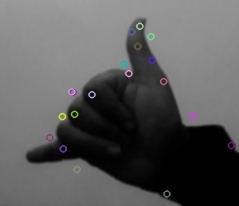
\includegraphics[width=.31\textwidth]{./Pictures/gesture/call_0_SIFT.jpg}
        }
        \subfigure[Closed Hand]{
           \label{fig:sift_2}
           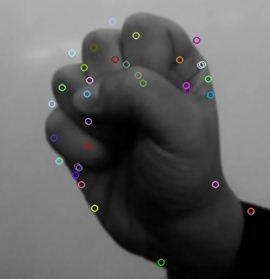
\includegraphics[width=.31\textwidth]{./Pictures/gesture/closed_10_SIFT.jpg}
        }
        \subfigure[Hand pointing to left]{
            \label{fig:sift_3}
            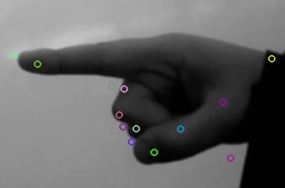
\includegraphics[width=.31\textwidth]{./Pictures/gesture/left_0_SIFT.jpg}
       }
   }
   \caption{SIFT features \label{fig:sift_example} }   
\end{dBox}   
\end{figure*}
\bigskip

\subsubsection{K-Means Clustering} \index{K-Means Clustering}
Clustering divides a group into subgroups, called clusters, so that the elements in the 
same cluster are similar. It is implemented using an unsupervised learning algorithm and an 
ordinary method for statistical data analysis applied in several fields, such as machine learning, 
pattern recognition, image analysis, data mining, and bioinformatics.
\bigskip

The number of clusters (the codebook size) depends on the structure of 
the data. There will be a compromise for how to choose the vocabulary size or number of 
clusters. If it is too small, then each bag-of-words vector will not represent all of the keypoints 
extracted from its related image. If it is too large, it will lead to overfitting because of insufficient 
samples of the keypoints extracted from the training image. 
We trained the classifier using 234 images with number of bags equal to 200. This number provides the most accurate recognition rate by trying different values \cite{Dardas11}.

\bigskip
The first step in k-means clustering is to divide the vector space (128-dimensional feature 
vector) into k clusters. K-means clustering starts with k randomly located centroids (points in space that represent the center of the cluster) and assigns every keypoint to the nearest one. After 
the assignment, the centroids (codevectors) are shifted to the average location of all the 
keypoints assigned to them, and assignments are redone. This procedure repeats until the 
assignments stop changing.

\bigskip
Once this is done, each feature vector (keypoint) is assigned to one and only one cluster 
center that is in the nearest distance with respect to the Euclidean distance metric in the 128-
dimensional feature vectors. The keypoints that are assigned to the same cluster center will be in 
the same subgroup so that after clustering, we have k disjoint subgroups of keypoints. Therefore, 
k-means clustering decreases the dimensionality for every training image with n keypoints 
(nx128) to 1xk, where k is the number of clusters.


\subsubsection{Classification} \index{Classification}
All the keypoints recovered in the training images are mapped with its generated bag-of-
words vector using k-means clustering. Then, all bag-of-words vectors with their related class or 
label numbers are fed into classifier. The following Algorithm \ref{bof-SIFT} sums up the whole process. \begin{algorithm}

\begin{dBox}
	\caption{Bag-of-Features SIFT Clustering} \label{bof-SIFT}
	\begin{algorithmic}[h]
		\Require{Dataset}
		\Ensure {Set of fixed attributes for each image}
		\Procedure{Bag-of-Features SIFT Clustering}{}
				\vspace{1em}	
				\State \emph{Stage 1: Obtain the set of bags of features.}
					\ForAll {images in the dataset}
						\State Extract the SIFT feature points.
						\State Obtain the SIFT descriptor the feature points extracted from the image.
					\EndFor
				\vspace{1em}	
				\State \emph{Stage 2: Clustering}
					\State Set the amount of bags to chosen number.
					\State Cluster the set of feature descriptors.
					\State Train the bags with K-Means Algorithm.
					\State Obtain the visual vocabulary.
		\EndProcedure	
	\end{algorithmic}
\end{dBox}	
\end{algorithm}
\bigskip
After the classifier is trained. For each new frame, SIFT features are extracted then clustered. Then the classifier is used to classifiy the clustered features. See the following Algorithm, Algorithm \ref{class-SIFT}
\begin{algorithm}[h]
\begin{dBox}
	\caption{Classification of given image} \label{class-SIFT}
	\begin{algorithmic}[1]
		\Require{Image}
		\Ensure {Gesture label if found}
		\Procedure{Classification of given image}{}
				\vspace{1em}	
				\State Extract SIFT feature points of the given image.
				\State Obtain SIFT descriptor for each feature point.
				\State Match the feature descriptors with the vocabulary we created in the first step
				\State Classifiy.

		\EndProcedure	
	\end{algorithmic}
\end{dBox}	
\end{algorithm}

\bigskip
 
Different classifiers were used and results were recorded. See chapter Limitations and classifications for more details.
\bigskip



\section{Dynamic Gestures}\index{Dynamic Gestures}
A lot of information can be extracted from time varying sequences of images, often more easily than from static images. In our case, a huge extension and variety of applications can be based on the detection of a moving hand. Camouflaged objects, the hand, are only easily seen when they move. Moreover, the relative sizes and position of objects are more easily determined when the objects move. Even simple image differencing provides an edge detector for the silhouettes of texture-free objects moving over any static background.\bigskip

The analysis of visual motion divides into two stages:
\begin{itemize}
\item The measurement of the motion, and 
\item The use of motion data to segment the scene into distinct objects and to extract two-dimensional information about the shape and motion of the objects \cite{dynamic1}.
\end{itemize}
\bigskip

There are two types of motion to consider; movement in the scene with a static camera, and movement of the camera, or ego motion. Since motion is relative anyway, these types of motion should be the same. However, this is not always the case, since if the scene moves relative to the illumination, shadow effects need to be dealt with. In addition, specularities can cause relative motion within the scene. For our work, we will ignore all such complications and focus on the first case which is having our hand moving before a static camera.\bigskip

When an object moves in front of a camera, there is a corresponding change in the image. Thus, if a point $p_0$ on an object moves with a velocity $v_0$, then the imaged point $p_i$ can be assigned a vector $v_i$ to indicate its movement on the image plane as Showen in Figure \ref{fig:dynamic12}(a). The collection of all these vectors forms the motion field.

\begin{figure*}[h]
\begin{dBox}
\centering
  \mbox{
      \subfigure[Point Moving in Image Plane]{
            \label{fig:dynamic_1}
            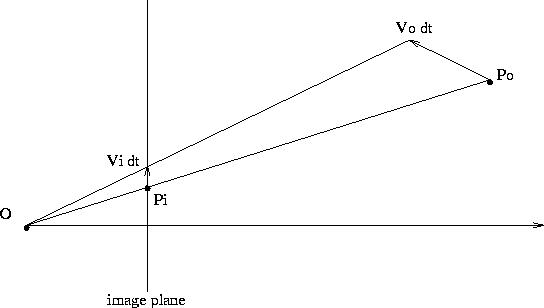
\includegraphics[width=.5\textwidth]{./Pictures/gesture/dynamic1.jpg}
        }
        \subfigure[Motion Field Idea]{
           \label{fig:dynamic_2}
           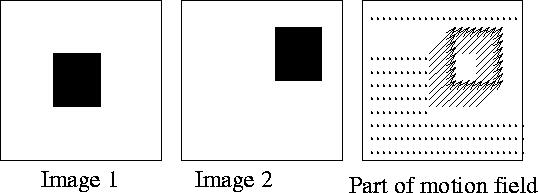
\includegraphics[width=.5\textwidth]{./Pictures/gesture/dynamic2.jpg}
        }
   }
   \caption{\label{fig:dynamic12} }   
\end{dBox}   
\end{figure*}

If we are only dealing with rigid body translations and rotations, then the motion field will be continuous except at the silhouette boundaries of objects.\bigskip

In the case of pure camera translation, the direction of motion as in Figure \ref{fig:dynamic12} (b) is along the projection ray through that image point from which (or towards which) all motion vectors radiate. The point of divergence (or convergence) of all motion field vectors is called the Focus Of Expansion FOE (or focus of contraction FOC). Thus, in the case of divergence we have forward motion of the camera, and in the case of convergence, backwards motion.\bigskip

If we take the axis of camera translation as the camera baseline in stereo, then every projection of a fixed scene point must translate along an epipolar line, and all such lines converge at the epipole, which is just the FOE \cite{dynamic2}.  Therefore, in order to track the motion we firstly need to determine the divergence field of optical flow motion.\bigskip


\subsection{Divergence Field and Optical Flow.}\index{Divergence Field and Optical Flow.}
In a vector field, divergence is an operator that measures the magnitude of the source or sink of the field. Given a vector $F=[F_1,F_2,..,F_n]^T$ in a n-dimensional Euclidean space, the divergence of F can be calculated as \bigskip

\begin{dBox}
\begin{equation}
DIVF = \sum_{i=1}^{n}\frac{d F_i}{d x_i}
\end{equation}
\end{dBox}

Where $[x1, x2, x3 … xn]$ T are the Cartesian coordinates of the space where the vector field is defined.\bigskip

Accordingly, for an optical flow vector field $F(x,y) = [u(x,y), v(x,y)]T$ where $u(x,y)$ and $v(x,y)$ are respectively the horizontal and vertical components of optical flow at position (x,y) the divergence of F is:

\begin{dBox}
\begin{equation}
divF = \frac{du}{dx} + \frac{dv}{dy}
\end{equation}
\end{dBox}
\bigskip

The following figures present an example of transforming s into a divergence field, where:

\begin{itemize}
\item Figure \ref{fig:dynamic345} (a,b) are Visualization of u and v respectively. 

\item Figure \ref{fig:dynamic345} (c) The corresponding Divergence Field after being normalized to gray-scale \cite{dynamic3}.

\end{itemize}


\begin{figure*}[h]
\begin{dBox}
\centering
  \mbox{
      \subfigure[]{
            \label{fig:dynamic_3}
            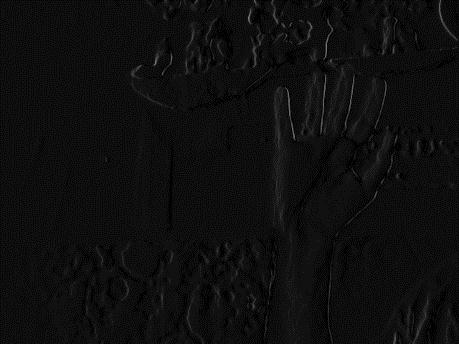
\includegraphics[width=.31\textwidth]{./Pictures/gesture/dynamic3.jpg}
        }
        \subfigure[]{
           \label{fig:dynamic_4}
           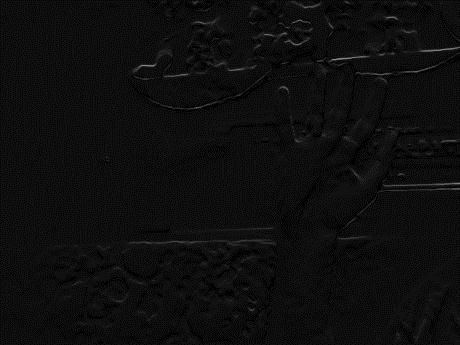
\includegraphics[width=.31\textwidth]{./Pictures/gesture/dynamic4.jpg}
        }
        \subfigure[]{
           \label{fig:dynamic_5}
           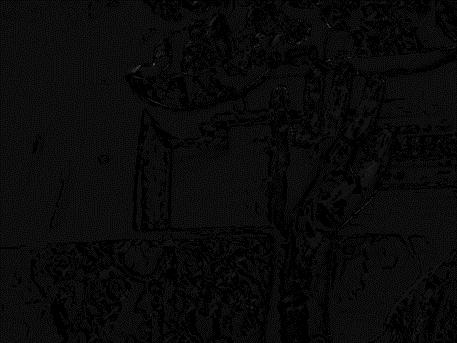
\includegraphics[width=.31\textwidth]{./Pictures/gesture/dynamic5.jpg}
        }
   }
   \caption{Example of transforming S into A divergence Field \label{fig:dynamic345} }   
\end{dBox}   
\end{figure*}
\bigskip

Then we use this as an input for Lucas Kanade Algorithm to calculate the Optical flow. In computer vision terms, Optical Flow is the image motion of objects as the objects, scene or camera, moves between two consecutive images. It is a 2D vector field of within-image translation. It is a classic and well-studied field in computer vision with many successful applications in for example video compression, motion estimation, object tracking and image segmentation.\bigskip

Optical flow relies on three major assumptions:
\begin{itemize}
\item 	Brightness constancy: The pixel intensities of an object in an image does not change between consecutive images.

\item  Temporal regularity: The between-frame time is short enough to consider the motion change between images using differentials (used to derive the central equation below).

\item  Spatial consistency: Neighboring pixels have similar motion.
\end{itemize}

In many cases these assumptions break down, but for small motions and short time steps between images it is a good model. Assuming that an object pixel I(x,y,t) at time t has the same intensity at time $t+\delta_t$ after motion $[\delta_x, \delta_y]$ means that 
\begin{dBox}
\begin{equation}
I(x,y,t) =I(x + \delta_{x,y} + \delta_{y,t} + \delta_t).
\end{equation}
\end{dBox}

Differentiating this constraint gives the optical flow equation:

\begin{dBox}
\begin{equation}
\bigtriangledown I^T V = - I_T.
\end{equation}
\end{dBox}

Where $V = [u, v]$ is the motion vector and It the time derivative. For individual points in the image, this equation is under-determined and cannot be solved (one equation with two unknowns in v). By enforcing some spatial consistency, it is possible to obtain solutions though. In the Lucas-Kanade algorithm below we will see how that assumption is used.\bigskip

The following figures show optical flow vectors (sampled at every $16^th$ pixel) shown on video of a waving hand \cite{dynamic4}. 

\begin{figure*}[h]
\begin{dBox}
\centering
  \mbox{
      \subfigure[]{
            \label{fig:dynamic_6}
            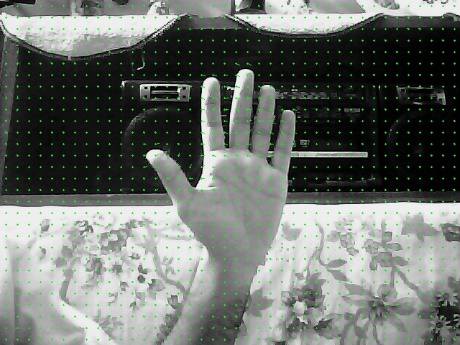
\includegraphics[width=.31\textwidth]{./Pictures/gesture/dynamic6.jpg}
        }
        \subfigure[]{
           \label{fig:dynamic_7}
           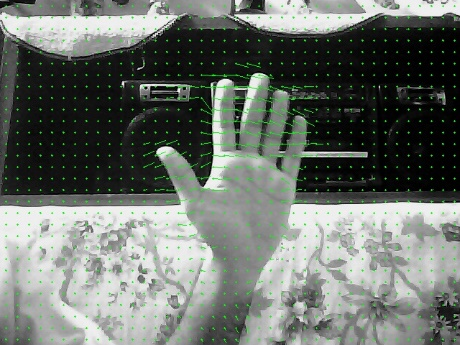
\includegraphics[width=.31\textwidth]{./Pictures/gesture/dynamic7.jpg}
        }
        \subfigure[]{
           \label{fig:dynamic_8}
           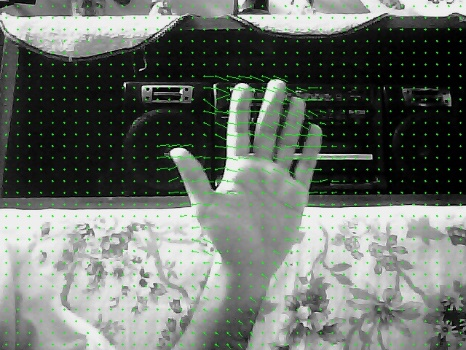
\includegraphics[width=.31\textwidth]{./Pictures/gesture/dynamic8.jpg}
        }
   }
   \caption{\label{fig:dynamic678} }   
\end{dBox}   
\end{figure*}

\begin{figure*}[h]
\begin{dBox}
\centering
  \mbox{
      \subfigure[]{
            \label{fig:dynamic_9}
            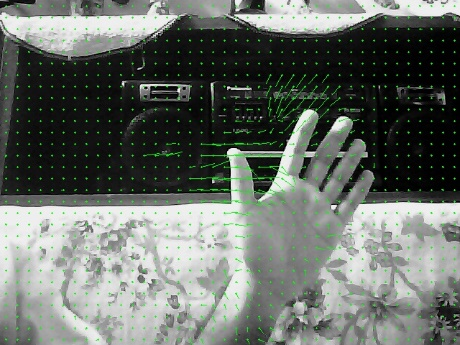
\includegraphics[width=.31\textwidth]{./Pictures/gesture/dynamic9.jpg}
        }
        \subfigure[]{
           \label{fig:dynamic_10}
           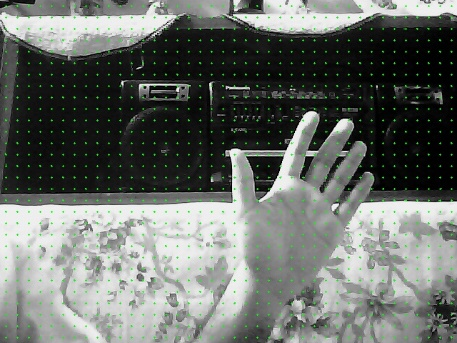
\includegraphics[width=.31\textwidth]{./Pictures/gesture/dynamic10.jpg}
        }
        \subfigure[]{
           \label{fig:dynamic_11}
           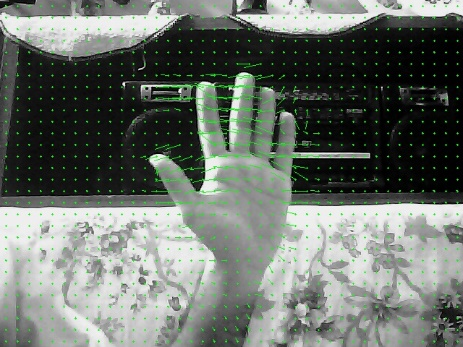
\includegraphics[width=.31\textwidth]{./Pictures/gesture/dynamic11.jpg}
        }
   }
   \caption{\label{fig:dynamic91011} }   
\end{dBox}   
\end{figure*}

\subsection{Lucas Kanade Algorithm \cite{dynamic4}}\index{Divergence Field and Optical Flow.}
Tracking is the process of following objects through a sequence of images or video. The most basic form of tracking is to follow interest points such as corners. A popular algorithm for this is the Lucas-Kanade tracking algorithm which uses a sparse optical flow algorithm. Lucas-Kanade tracking can be applied to any type of features but usually makes use of corner points similar to the Harris corner points \cite{dynamic6} .\bigskip

Depending on Harris corner points we find good feature points to track. These points are corners detected according to an algorithm by Shi and Tomasi \cite{dynamic7}  where corners are points with two large eigenvalues of the structure tensor (Harris matrix) and where the smaller eigenvalue is above a threshold.\bigskip

The optical flow equation is under-determined (meaning that there are too many unknowns per equation) if considered on a per-pixel basis. Using the assumption that neighboring pixels have the same motion it is possible to stack many of these equations into one system of equations\bigskip

For some neighborhood of n pixels. This has the advantage that the system now has more equations than unknowns and can be solved with least square methods. Typically, the contribution from the surrounding pixels is weighted so that pixels farther away have less influence. A Gaussian weighting is the most common choice.\bigskip

Standard Lucas-Kanade tracking works for small displacements. To handle larger displacements a hierarchical approach is used. In this case, the optical flow is computed at coarse to fine versions of the image. The following Figures shows the steps of Lucas-Kanade Tracking Algorithm. First by detecting the feature points in the first image and then keep tracking the flow until the motion is 0 then draws where the feature points have stopped. \bigskip

\begin{figure*}[h]
\begin{dBox}
\centering
  \mbox{
      \subfigure[]{
            \label{fig:dynamic_12}
            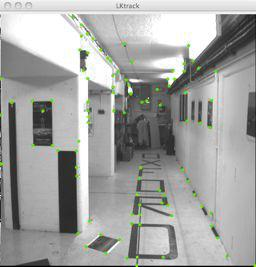
\includegraphics[width=.31\textwidth]{./Pictures/gesture/dynamic12.jpg}
        }
        \subfigure[]{
           \label{fig:dynamic_13}
           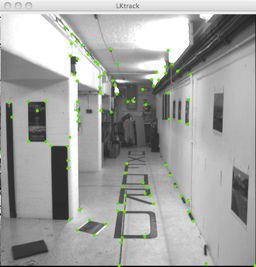
\includegraphics[width=.31\textwidth]{./Pictures/gesture/dynamic13.jpg}
        }
        \subfigure[]{
           \label{fig:dynamic_14}
           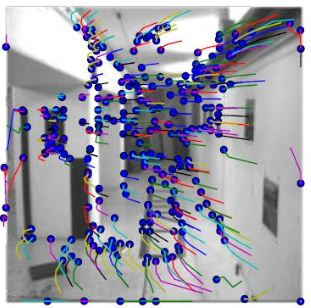
\includegraphics[width=.31\textwidth]{./Pictures/gesture/dynamic14.jpg}
        }
   }
   \caption{\label{fig:dynamic121314} }   
\end{dBox}   
\end{figure*}

From this stage, our algorithm exploits the Lucas-Kanade Algorithm and takes a very simple turn. Based on the assumption mentioned at the beginning of the chapter, we only have four directions for the motion; Up, Down, Right Left. The simplicity of our dynamic gestures alleviated the processing overhead gigantically and yet made great use of the output of Lucas-Kanade Algorithm.\bigskip

From Lucas-Kanade Algorithm we get an output as 2D array. This 2D array contains the new positions for the detected feature point as tracked. Given that we already have the original indices of these feature points. We can get the difference between the coordinates of the new positions and the old ones.\bigskip

From Lucas-Kanade Algorithm we get an output as 2D array. This 2D array contains the new positions for the detected feature point as tracked. Given that we already have the original indices of these feature points. We can get the difference between the coordinates of the new positions and the old ones.\bigskip

To decide that the hand has moved, the difference between the new position and the new one must exceed a given threshold. If the hand even slightly moved and the difference is less than the threshold it is considered static until the movement exceeds the threshold then the detection starts. This threshold is applied to the vertical and horizontal motion components for ever feature point. If the x or the horizontal motion difference exceeded the threshold then the hand object moved horizontally. The same applies to y or the vertical component. If both differences at the x and y components didn’t exceed the threshold, then this feature points hadn’t move.\bigskip


The following flowchart explains what happens at each feature point, where $I(x,y)$ is the original indices for a feature point and $I'(x',y')$ the new indices in the new image after the movement. \bigskip

\begin{figure*}[h]
\begin{dBox}
\centering
  \mbox{
      \subfigure[]{
            \label{fig:dynamic_15}
            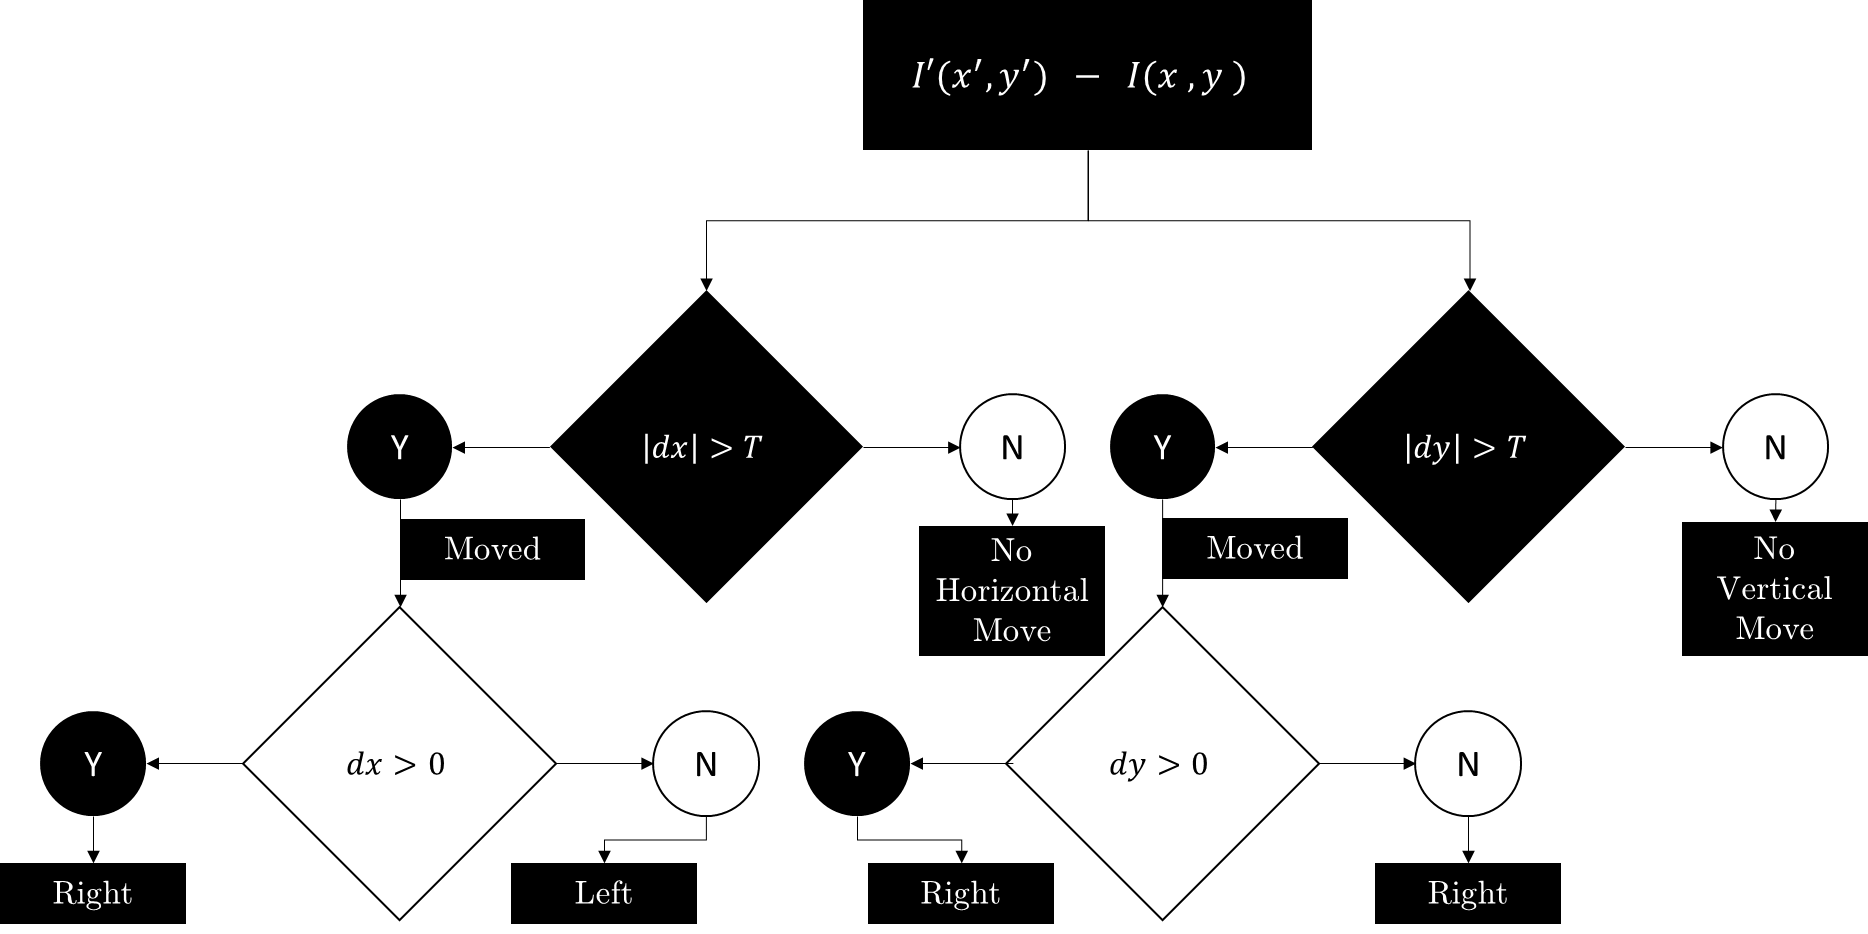
\includegraphics[width=.9\textwidth]{./Pictures/gesture/dynamic15.png}
        }
        
   }
   \caption{Flow Chart\label{fig:dynamic15} }   
\end{dBox}   
\end{figure*}

Then we check the difference itself if it is indicating that the hand moved if the direction is to the positive side of each axes or differently in the negative one. We have four counters to help in determining the direction. Each counter is increased at each feature point in the direction this point moved to.\bigskip


According to these two steps of the flowchart at each feature point one or two of the four counters are increased. This includes if a point moved in two directions i.e. bottom left. The point that according to the movement to the right, left up or down, the majority of points will vote correctly and the counter of the correct direction will always be greater than the rest. \bigskip

\subsection{Integration with Static Gesture Recognition}\index{Divergence Field and Optical Flow.}
The Gesture Recognition Process always starts with simple static gesture recognition. The recognition of the static gestures goes smoothly until the up-index finger appear before the camera. This signals the detection of a dynamic gesture coming next. The algorithm then wait for another frame with the same gesture but with its feature points moved to another location. The algorithm keeps taking frames of the dynamic gestures, applying optical flow algorithm for every two consecutive frames. Consequently, it stores the direction until there is no motion between the upcoming frames (up to three frames with no motion).Then, take the action according to the majority of the saved directions.\bigskip


The handling of static gestures can be reactivated once more, if the separator appeared which indicates a change of gestures. The dynamic gestures has no separator as long as you keep going in front of the camera your motions gets recorded and interpreted according to the application.\bigskip


The following diagram illustrates these transitions:

\begin{figure*}[h]
\begin{dBox}
\centering
  \mbox{
      \subfigure[]{
            \label{fig:dynamic_16}
            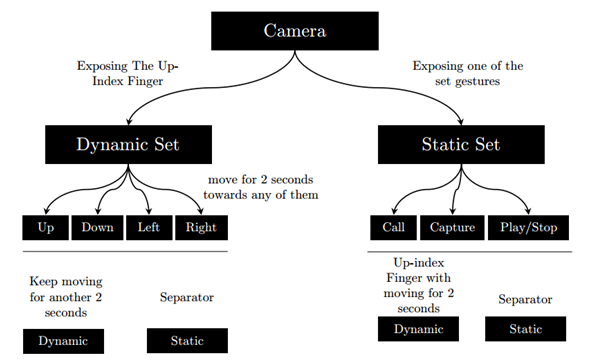
\includegraphics[width=.8\textwidth]{./Pictures/gesture/dynamic16.png}
        }
        
   }
   \caption{Transition Diagram Between Static and Dynamic Gestures\label{fig:dynamic16} }   
\end{dBox}   
\end{figure*}

\section{Limitations and Classification}\index{Limitations and Classification}
This chapter includes the work done to detect static gestures. It begins by describing the general idea of segmentation and recognition and then proceeds to the following sections.\bigskip

\subsection{Assumptions and Limitations}\index{Assumptions and Limitations}
Not Yet \bigskip

\subsection{Classification} \index{Classification}
Our Dataset of gestures contains exactly 234 images. These images are different views for our 8 gestures. Every view is represented as a 1-D Array. The group of images or views is acting as a reference for the classifier to check every query image against it. For every gesture there is a label that the classifier, when its job is done, decides, according to this classifier’s algorithm, to which label the query image belongs. The following is our gestures and with how many views they are represented in the dataset:

\paragraph{Start Gesture}\index{Classification}
The gesture is represented by the Ok sign (3 fingers) as shown in Figure \ref{fig:set1} (a). This gesture is marking the start of the detection for any gesture to come forth. It is represented with 18 views in the dataset.

\paragraph{Open Hand}\index{Classification}
This gesture is represented by the full hand opened and exposed to the camera as show in Figure \ref{fig:set1} (b). This gesture can be interpreted in many ways according to the application. For example, stop and play in music player. In the dataset, this gesture is represented by 22 views including left and right hands.

\paragraph{Closed Hand}\index{Classification}
This gesture is represented by the full hand closed, fist, and exposed to the camera as show in Figure \ref{fig:set1}(c). This gesture has a special rule. It acts as a separator between the gestures detection i.e. if we detected a gesture, we cannot hope to detect one another following it until the algorithm, any of them receives the fist gesture. In the dataset, this gesture is represented by 14 views.

\paragraph{Capture Gesture}\index{Classification}
This gesture is represented by a hand shaping a letter C as show in Figure \ref{fig:set1}(d). This gesture has a specific need which is to signal the camera to be opened for capturing an image and capturing after the camera is running. In the dataset, this gesture is represented by 54 view including left and right hands. 

\begin{figure*}[h]
\begin{dBox}
\centering
  \mbox{
      \subfigure[Start Gesture]{
            \label{fig:ok}
            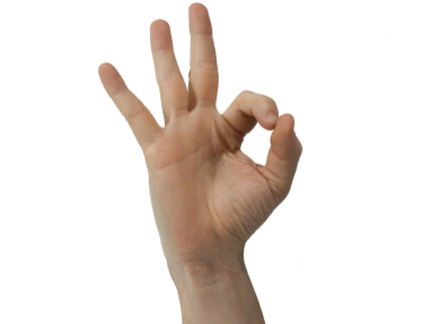
\includegraphics[width=.31\textwidth]{./Pictures/gesture/ok.jpg}
        }
        \subfigure[Open Hand Gesture]{
           \label{fig:open_g}
           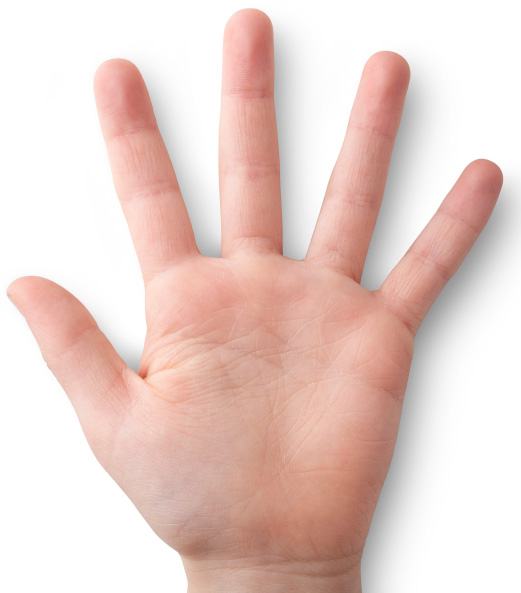
\includegraphics[width=.25\textwidth]{./Pictures/gesture/open.jpg}
        }
        \subfigure[Closed Hand Gesture]{
            \label{fig:closed_g}
            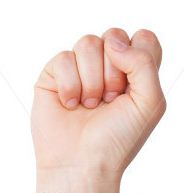
\includegraphics[width=.28\textwidth]{./Pictures/gesture/closed.jpg}
       }
        \subfigure[Capture Gesture]{
            \label{fig:capture_g}
            \includegraphics[width=.31\textwidth]{./Pictures/gesture/capture.jpg}
       }
   }
   \caption{Defined Gestures Set 1 \label{fig:set1} }   
\end{dBox}   
\end{figure*}

\paragraph{Call Gesture}\index{Classification}
This gesture is represented by the thumb and the little finger and exposed to the camera as show in Figure \ref{fig:set2}(a). This gesture is used specifically to open the dialer or actually signal to call a number. In the dataset, this gesture is represented by 31 view including left and right hands.

\paragraph{Up Gesture}\index{Classification}
This gesture is represented index finger pointing up and exposed to the camera as show in Figure \ref{fig:set2}(b). This gesture has a special role in our set. It marks the start of detecting a dynamic gesture as mentioned in the dynamic gesture chapter. In the dataset, this gesture is represented by 24 view including left and right hands. 

\paragraph{Right Gesture}\index{Classification}
This gesture is represented by the thumb pointing to the right and exposed to the camera as show in Figure \ref{fig:set2}(c). This gesture can be interpreted in many ways according to the application. For example, stop and play in music player. In the dataset, this gesture is represented by 30 views. 

\paragraph{Left Gesture}\index{Classification}
This gesture is represented by the thumb pointing to the left and exposed to the camera as show in Figure \ref{fig:set2}(d). This gesture can be interpreted in many ways according to the application. For example, stop and play in music player. In the dataset, this gesture is represented by 22 views.

\begin{figure*}[h]
\begin{dBox}
\centering
  \mbox{
      \subfigure[Call Gesture]{
            \label{fig:call}
            \includegraphics[width=.31\textwidth]{./Pictures/gesture/call.jpg}
        }
        \subfigure[Up Gesture]{
           \label{fig:up_g}
           \includegraphics[width=.23\textwidth]{./Pictures/gesture/up.jpg}
        }
        \subfigure[Right Gesture]{
            \label{fig:right_g}
            \includegraphics[width=.31\textwidth]{./Pictures/gesture/right.jpg}
       }
        \subfigure[Left Gesture]{
            \label{fig:left_g}
            \includegraphics[width=.23\textwidth]{./Pictures/gesture/left.jpg}
       }
   }
   \caption{Defined Gestures Set 2 \label{fig:set2} }   
\end{dBox}   
\end{figure*}

Every algorithm from the previous chapter passes a 1-D array to the classifier. This 1-D array is the classifier input. In the following sections, we are going to represent the three classifiers we used, for our work and how they use this 1-D array. \bigskip

\subsubsection{Support Vector Machine}\index{Support Vector Machine}
SVM method for the classification of both linear and nonlinear data \cite{classifications}. The algorithm works as follows. It uses a nonlinear mapping to transform the original training data into a higher dimension. Within this new dimension, it searches for the linear optimal separating hyperplane (i.e., a “decision boundary” separating the tuples of one class from another). With an appropriate nonlinear mapping to a sufficiently high dimension, data from two classes can always be separated by a hyperplane. The SVM finds this hyperplane using support vectors (“essential” training tuples) and margins (defined by the support vectors).We will delve more into these new concepts later.


Although the training time of even the fastest SVMs can be extremely slow, they are highly accurate, owing to their ability to model complex nonlinear decision boundaries. They are much less prone to overfitting than other methods. The support vectors found also provide a compact description of the learned model. SVMs can be used for numeric prediction as well as classification. They have been applied to a number of areas, including handwritten digit recognition, object recognition, and speaker identification, as well as benchmark time-series prediction tests.
 \bigskip
\paragraph{Linear Separability Of The Data}
To explain the mystery of SVMs, let’s first look at the simplest case; a two-class problem where the classes are linearly separable. Let the data set D be given as (X1, y1),
(X2, y2), … , (XD, yD), where Xi is the set of training tuples with associated class labels, yi. Each yi can take one of two values, either +1 or -1 (i.e., $yi \subseteq{+1,-1}$), corresponding to the classes buys computer D yes and buys computer D no, respectively.\bigskip

To aid in visualization, let’s consider an example based on two input attributes, A1 and A2, as shown in Figure \ref{fig:svm1}. From the graph, we see that the 2-D data are linearly separable (or “linear,” for short), because a straight line can be drawn to separate all the tuples of class +1 from all the tuples of class -1.\bigskip

\begin{figure*}[h]
\begin{dBox}
\centering
  \mbox{
      \subfigure[]{
            \label{fig:svm_1}
            \includegraphics[width=.31\textwidth]{./Pictures/gesture/svm1.jpg}
        }
   }
   \caption{SVM Separability Idea\label{fig:svm1} }   
\end{dBox}   
\end{figure*}

There are an infinite number of separating lines that could be drawn. We want to find the “best” one, that is, one that will have the minimum classification error on previously unseen tuples. How can we find this best line? Note that if our data were 3-D (i.e., with three attributes); we would want to find the best separating plane. Generalizing to n dimensions, we want to find the best hyperplane. We will use “hyperplane” to refer to the decision boundary that we are seeking, regardless of the number of input attributes.\bigskip

An SVM approaches this problem by searching for the maximum marginal hyperplane. Consider Figure \ref{fig:svm2}, which shows two possible separating hyperplanes and their associated margins. Before we get into the definition of margins, let’s take an intuitive look at this figure. Both hyperplanes can correctly classify all the given data tuples. Intuitively, however, we expect the hyperplane with the larger margin to be more accurate at classifying future data tuples than the hyperplane with the smaller margin. This is why (during the learning or training phase) the SVM searches for the hyperplane with the largest margin, that is, the maximum marginal hyperplane (MMH). The associated margin gives the largest separation between classes.
\bigskip
\begin{figure*}[h]
\begin{dBox}
\centering
  \mbox{
      \subfigure[]{
            \label{fig:svm_2}
            \includegraphics[width=.8\textwidth]{./Pictures/gesture/svm2.jpg}
        }
   }
   \caption{SVM With Possible Separating hyperplanes\label{fig:svm2} }   
\end{dBox}   
\end{figure*}

Getting to an informal definition of margin, we can say that the shortest distance from a hyperplane to one side of its margin is equal to the shortest distance from the hyperplane to the other side of its margin, where the “sides” of the margin are parallel to the hyperplane. When dealing with the MMH, this distance is, in fact, the shortest distance from the MMH to the closest training tuple of either class. A separating hyperplane can be written as $W.X+b = 0 $ Where W is a weight vector, namely, W =${  w_1,w_2,…,w_n }$; n is the number of attributes; and b is a scalar, often referred to as a bias. To aid in visualization, let’s consider two input attributes, A1 and A2, as in Figure \ref{fig:svm2} (b). Training tuples are 2-D (e.g., X = (x1, x2)), where x1 and x2 are the values of attributes A1 and A2, respectively, for X. If we think of b as an additional weight, w0, we can rewrite the previous equation as $w_{0} + w_{1} x_{1}+w_{2} x_{2}=0$ \bigskip

Thus, any point that lies above the separating hyperplane satisfies

\begin{dBox}
\begin{equation}
w_0 + w_1 x_1 + w_2  x_2 > 0 
\end{equation}
\end{dBox}

Similarly, any point that lies below the separating hyperplane satisfies

\begin{dBox}
\begin{equation}
w_0 + w_1 x_1 + w_2  x_2 < 0 
\end{equation}
\end{dBox}

The weights can be adjusted so that the hyperplanes defining the “sides” of the margin can be written as

\begin{dBox}
\begin{equation}
H_1: w_0 + w_1 x_1 + w_2 x_2 >= 1    $ for $  y_i = +1,
\end{equation}
\begin{equation}
H_2: w_0 + w_1 x_1 + w_2 x_2 =< -1    $ for $ y_i = -1
\end{equation}
\end{dBox}

That is, any tuple that falls on or above H1 belongs to class +1, and any tuple that falls on or below H2 belongs to class -1. Combining the two inequalities:

\begin{dBox}
\begin{equation}
y_{i}(w_0 + w_1 x_1 + w_2 x_2) >= 1 $ for all i$. 
\end{equation}
\end{dBox}
\bigskip
Any training tuples that fall on hyperplanes H1 or H2 (i.e., the “sides” defining the margin) satisfy the previous equation and are called support vectors. That is, they are equally close to the (separating) MMH. In \ref{fig:svm3}, the support vectors are shown encircled with a thicker border. Essentially, the support vectors are the most difficult tuples to classify and give the most information regarding classification.\bigskip
\bigskip
\begin{figure*}[h]
\begin{dBox}
\centering
  \mbox{
      \subfigure[]{
            \label{fig:svm_3}
            \includegraphics[width=.8\textwidth]{./Pictures/gesture/svm3.jpg}
        }
   }
   \caption{Higlight Support Vectors\label{fig:svm3} }   
\end{dBox}   
\end{figure*}

From this, we can obtain a formula for the size of the maximal margin. The distance from the separating hyperplane to any point on H1 is $1/|(|W|)|$, where $|(|W|)|$ is the Euclidean norm of W, that is, $\sqrt{W . W2}$. By definition, this is equal to the distance from any point on H2 to the separating hyperplane. Therefore, the maximal margin is $2/|(|W|)|$. Using some “fancy math tricks,” we can rewrite the last equation so that it becomes what is known as a constrained (convex) quadratic optimization problem. Note that the tricks involve rewriting the last equation using a Lagrangian formulation and then solving for the solution using Karush-Kuhn-Tucker (KKT) conditions. If the data are small (say, less than 2000 training tuples), any optimization software package for solving constrained convex quadratic problems can then be used to find the support vectors and MMH. For larger data, special and more efficient algorithms for training SVMs can be used instead. Once we’ve found the support vectors and MMH (note that the support vectors define the MMH!), we have a trained support vector machine. The MMH is a linear class boundary, and so the corresponding SVM can be used to classify linearly separable data. We refer to such a trained SVM as a linear SVM.\bigskip

Based on the Lagrangian formulation mentioned before, the MMH can be rewritten as the decision boundary;

\begin{dBox}
\begin{equation}
d(X^{T}) = \sum_{i=1}^{l}{y_i \alpha_i X_i X^T} + b_0
\end{equation}
\end{dBox}

Where $y_i$  is the class label of support vector $X_i$ , $X^T$ is a test tuple; $\alpha_i$ and $b_0$ are numeric parameters that were determined automatically by the optimization or SVM algorithm noted before; and l is the number of support vectors. $\alpha_i$ are Lagrangian multipliers. For linearly separable data, the support vectors are a subset of the actual training tuples (although there will be a slight twist regarding this when dealing with non linearly separable data, as we shall see in the following).\bigskip

Given a test tuple, $X^T$, we plug it into last equation and then check to see the sign of the result. This tells us on which side of the hyperplane the test tuple falls. If the sign is positive, then $X^T$  falls on or above the MMH, and so the SVM predicts that $X^T$  belongs to class +1 (representing buys computer = yes, in our case). If the sign is negative, then $X^T$  falls on or below the MMH and the class prediction is -1 (representing buys computer = no). Notice that the Lagrangian formulation of our problem from the last equation contains a dot product between support vector $X_i$ and test tuple $X^T$. This will prove very useful for finding the MMH and support vectors for the case when the given data are non linearly separable, as described further in the next section. Before we move on to the nonlinear case, there are two more important things to note. The complexity of the learned classifier is characterized by the number of support vectors rather than the dimensionality of the data. Hence, SVMs tend to be less prone to overfitting than some other methods. The support vectors are the essential or critical training tuples—they lie closest to the decision boundary (MMH). If all other training tuples were removed and training were repeated, the same separating hyperplane would be found. Furthermore, the number of support vectors found can be used to compute an (upper) bound on the expected error rate of the SVM classifier, which is independent of the data dimensionality. An SVM with a small number of support vectors can have good generalization, even when the dimensionality of the data is high.

\paragraph{Linear In-separability Of The Data}
The approach described for linear SVMs can be extended to create nonlinear SVMs for the classification of linearly inseparable data (also called nonlinearly separable data, or nonlinear data for short). Such SVMs are capable of finding nonlinear decision boundaries (nonlinear hypersurfaces) in input space. We obtain a nonlinear SVM by extending the approach for linear SVMs as follows. There are two main steps. In the first step, we transform the original input data into a higher dimensional space using a nonlinear mapping. Several common nonlinear mappings can be used in this step, as we will further describe next. Once the data have been transformed into the new higher space, the second step searches for a linear separating hyperplane in the new space. We again end up with a quadratic optimization problem that can be solved using the linear SVM formulation. The maximal marginal hyperplane found in the new space corresponds to a nonlinear separating hypersurface in the original space.\bigskip
\begin{figure*}[h]
\begin{dBox}
\centering
  \mbox{
      \subfigure[]{
            \label{fig:svm_4}
            \includegraphics[width=.8\textwidth]{./Pictures/gesture/svm4.jpg}
        }
   }
   \caption{Linear In-separable Data\label{fig:svm4} }   
\end{dBox}   
\end{figure*}

However, there are some problems. First, how do we choose the nonlinear mapping to a higher dimensional space? Second, the computation involved will be costly. Referring to the last equation, for the classification of a test tuple, $X^T$. Given the test tuple, we have to compute its dot product with every one of the support vectors. In training, we have to compute a similar dot product several times in order to find the MMH. This is especially expensive. Hence, the dot product computation required is very heavy and costly.\bigskip

We can use another math trick. It so happens that in solving the quadratic optimization problem of the linear SVM (i.e., when searching for a linear SVM in the new higher dimensional space), the training tuples appear only in the form of dot products, $\phi{x_i }) $ .$\phi{x_j } $ , where $\phi{x_i }) $ is simply the nonlinear mapping function applied to transform the training tuples. Instead of computing the dot product on the transformed data tuples, it turns out that it is mathematically equivalent to instead apply a kernel function, $K(x_i,x_j )$  to the original input data. That is:
\begin{dBox}
\begin{equation}
K(x_i,x_j) = \phi{x_i} \phi{x_j}.
\end{equation}
\end{dBox}

In other words, everywhere that $\phi{x_i}$.$\phi{x_j}.$appears in the training algorithm, we can replace it with $K(x_i,x_j )$. In this way, all calculations are made in the original input space, which is of potentially much lower dimensionality! We can safely avoid the mapping—it turns out that we don’t even have to know what the mapping is! We will talk more later about what kinds of functions can be used as kernel functions for this problem.

After applying this trick, we can then proceed to find a maximal separating hyperplane.\bigskip

Properties of the kinds of kernel functions that could be used to replace the dot product scenario just described have been studied. Three admissible kernel functions are:

\begin{itemize}
\item Polynomial kernel of degree $h: K(x_i,x_j )=(x_i.x_j+1)^h$.
\item Gaussian radial basis function kernel: $K(x_i,x_j )=e^-\frac{\|x_i- x_j \|^2}{2\sigma^2}$.
\item Sigmoid kernel: $K(x_i,x_j )=tanh(x_i.x_i-\delta)$.
\end{itemize}

Each of these results in a different nonlinear classifier in (the original) input space. Neural network aficionados will be interested to note that the resulting decision hyperplanes found for nonlinear SVMs are the same type as those found by other well-known neural network classifiers. For instance, an SVM with a Gaussian radial basis function (RBF) gives the same decision hyperplane as a type of neural network known as a radial basis function network. An SVM with a sigmoid kernel is equivalent to a simple two-layer neural network known as a multilayer perceptron (with no hidden layers). \bigskip

There are no golden rules for determining which admissible kernel will result in the most accurate SVM. In practice, the kernel chosen does not generally make a large difference in resulting accuracy. SVM training always finds a global solution, unlike neural networks, such as back propagation.
\bigskip

So far, we have described linear and nonlinear SVMs for binary (i.e., two-class) classification. SVM classifiers can be combined for the multiclass case.  A major research goal regarding SVMs is to improve the speed in training and testing so that SVMs may become a more feasible option for very large data sets (e.g., millions of support vectors). Other issues include determining the best kernel for a given data set and finding more efficient methods for the multiclass case.\bigskip

SVM has the following results on our datasets. For Binary Representation Algorithm, it gives the best results according to the following results that describe the accuracy of ever static algorithm. \bigskip

\begin{figure*}[h]
\begin{dBox}
\centering
  \mbox{
      \subfigure[]{
            \label{fig:r_svm_b}
            \includegraphics[width=.9\textwidth]{./Pictures/gesture/R_SVM_Binary.jpg}
        }
   }
   \caption{Binary Based Approach Results Using x-validation with k=10\label{fig:r_svm_b} }   
\end{dBox}   
\end{figure*}

\begin{figure*}[h]
\begin{dBox}
\centering
  \mbox{
      \subfigure[]{
            \label{fig:r_svm_f}
            \includegraphics[width=.9\textwidth]{./Pictures/gesture/R_SVM_Feature.jpg}
        }
   }
   \caption{Feature Based Approach Results Using x-validation with k=10\label{fig:r_svm_f} }   
\end{dBox}   
\end{figure*}


\subsubsection{Naïve Base}\index{Naïve Base}
Not Yet \bigskip

\subsubsection{KNN}\index{KNN}
The k-nearest-neighbor method \cite{classifications} was first described in the early 1950s. The method is labor intensive when given large training sets, and did not gain popularity until the 1960s when increased computing power became available. It has since been widely used in the area of pattern recognition. \bigskip

Nearest-neighbor classifiers are based on learning by analogy, that is, by comparing a given test tuple with training tuples that are similar to it. The training tuples are described by n attributes. Each tuple represents a point in an n-dimensional space. In this way, all the training tuples are stored in an n-dimensional pattern space.When given an unknown tuple, a k-nearest-neighbor classifier searches the pattern space for the k training tuples that are closest to the unknown tuple. These k training tuples are the k “nearest neighbors” of the unknown tuple.
\bigskip

“Closeness” is defined in terms of a distance metric, such as Euclidean distance. The
Euclidean distance between two points or tuples, say, $X1 =( x_{11}, x_{12},..., x_{1n})$ and $X2=(x_{21}, x_{22},..., x_{2n})$, is

\begin{dBox}
\begin{equation}
dist(x_1, x_2) = \sqrt{\sum_{i=1}^{n}(x_{1i}-x_{2i})^2}
\end{equation}
\end{dBox}


For k-nearest-neighbor classification, the unknown tuple is assigned the most common class among its k-nearest neighbors. When k = 1, the unknown tuple is assigned the class of the training tuple that is closest to it in pattern space. Nearest-neighbor classifiers can also be used for numeric prediction, that is, to return a real-valued prediction
for a given unknown tuple. In this case, the classifier returns the average value of the real-valued labels associated with the k-nearest neighbors of the unknown tuple.\bigskip

The previous discussion assumes that the attributes used
to describe the tuples are all numeric. For nominal attributes, a simple method is to compare the corresponding value of the attribute in tuple X1 with that in tuple X2. If
the two are identical (tuples X1 and X2 both have the color blue), then the difference between the two is taken as 0. If the two are different ( tuple X1 is blue but tuple X2 is red), then the difference is considered to be 1. Other methods may incorporate more sophisticated schemes for differential grading (where a larger difference score is assigned, say, for blue and white than for blue and black).\bigskip

“How can I determine a good value for k, the number of neighbors?” This can be determined experimentally. Starting with k = 1, we use a test set to estimate the error rate
of the classifier. This process can be repeated each time by incrementing k to allow for one more neighbor. The k value that gives the minimum error rate may be selected. In
general, the larger the number of training tuples, the larger the value of k will be (so that classification and numeric prediction decisions can be based on a larger portion of the stored tuples). As the number of training tuples approaches infinity and k = 1, the error rate can be no worse than twice the Bayes error rate (the latter being the theoretical minimum). If k also approaches infinity, the error rate approaches the Bayes error rate.\bigskip

Nearest-neighbor classifiers can be extremely slow when classifying test tuples. If D is a training database of |D| tuples and k = 1, then O(|D|) comparisons are required to
classify a given test tuple. By presorting and arranging the stored tuples into search trees, the number of comparisons can be reduced to O(log|D|). Parallel implementation can
reduce the running time to a constant, that is, O(1), which is independent of |D|. Other techniques to speed up classification time include the use of partial distance
calculations and editing the stored tuples. In the partial distance method, we compute the distance based on a subset of the n attributes. If this distance exceeds a threshold,
then further computation for the given stored tuple is halted, and the process moves on to the next stored tuple. The editing method removes training tuples that prove useless. This method is also referred to as pruning or condensing because it reduces the total
number of tuples stored.\bigskip

K-NN has the following results on our datasets. For Binary Representation Algorithm, it gives the best results according to the following results that describe the accuracy of ever static algorithm.\bigskip

\begin{figure*}[h]
\begin{dBox}
\centering
  \mbox{
      \subfigure[]{
            \label{fig:r_knn_b}
            \includegraphics[width=.9\textwidth]{./Pictures/gesture/R_K-NN_B.jpg}
        }
   }
   \caption{Binary Based Approach Results Using x-validation with k=10\label{fig:r_knn_b} }   
\end{dBox}   
\end{figure*}

\begin{figure*}[h]
\begin{dBox}
\centering
  \mbox{
      \subfigure[]{
            \label{fig:r_knn_f}
            \includegraphics[width=.9\textwidth]{./Pictures/gesture/R_K-NN_F.jpg}
        }
   }
   \caption{Feature Based Approach Results Using x-validation with k=10\label{fig:r_knn_f} }   
\end{dBox}   
\end{figure*}
